 % arara: pdflatex: { synctex: yes }
% arara: makeindex: { style: ctuthesis }
% arara: bibtex

% The class takes all the key=value arguments that \ctusetup does,
% and a couple more: draft and oneside
\documentclass[twoside]{ctuthesis}
\usepackage{graphicx}
\usepackage{adjustbox}
\usepackage{makecell}
\usepackage[colorinlistoftodos]{todonotes}
\usepackage[sortlocale=cs_CZ, sorting=debug, style=iso-numeric, maxnames=2]{biblatex}
\usepackage{array,etoolbox}
\usepackage{xcolor}
\usepackage{caption}
\usepackage{subcaption}
\usepackage{enumitem}
\usepackage{multirow}
\usepackage{multicol}
\usepackage{chngpage}
\usepackage{rotating}
\usepackage{empheq}
\usepackage{color, colortbl}
\usepackage[acronym,nomain,nonumberlist]{glossaries}
\makenoidxglossaries

\renewcommand{\glossarysection}[2][]{}

\newacronym{ui}{UI}{Uživatelské rozhraní}
\newacronym{dpp}{DPP}{Dohoda o~provedení práce}
\newacronym{dpc}{DPČ}{Dohoda o~pracovní činnosti}
\newacronym{mvc}{MVC}{Model-View-Controller}
\newacronym{mvvm}{MVVM}{Model-View-ViewModel}
\newacronym{uc}{UC}{Use Case (případ užití)}
\newacronym{dao}{DAO}{Data Access Object}
\newacronym{rest}{REST}{Representational state transfer}
\newacronym{api}{API}{Application Programming Interface}


\newacronym{json}{JSON}{JavaScript Object Notation}
\newacronym{crud}{CRUD}{Create, Read, Update, Delete}
\newacronym{html}{HTML}{Hypertext Markup Language}
\newacronym{xml}{XML}{Extensible Markup Language}
\newacronym{sql}{SQL}{Structured Query Language}
\newacronym{orm}{ORM}{Object Relation Mapping}
\newacronym{id}{ID}{Identifikátor}

\newacronym{dsl}{DSL}{Domain-specific language}
\newacronym{http}{HTTP}{Hypertext Transfer Protocol}
\newacronym{url}{URL}{Uniform Resource Locator}
\newacronym{mvp}{MVP}{Model-View-Presenter}
\newacronym{ide}{IDE}{Integrated Development Environment}

\newacronym{rpc}{RPC}{Remote Procedure Call}
\usepackage{listings}

\definecolor{Gray}{gray}{0.9}

\newcommand{\coloredeq}[2]{\begin{empheq}[box=\colorbox{Gray}]{align}\label{#1}\hspace{1em}#2\hspace{1em}\end{empheq}}

\graphicspath{{img/}}

\preto\tabular{\setcounter{magicrownumbers}{0}}
\newcounter{magicrownumbers}
\newcommand\rownumber{\stepcounter{magicrownumbers}\arabic{magicrownumbers}}

\renewcommand*{\finalnamedelim}{ a }
\ctusetup{
	mainlanguage = czech,
	otherlanguages = {slovak, english},
	title-czech = {Mobilní aplikace pro plánování lidských zdrojů},
	title-english = {Mobile App for Human Resource Planning},
	doctype = B,
	faculty = F3,
	department-czech = {Katedra počítačů},
	department-english = {Department of Computer Science},
	author = {Martina Kopecká},
	supervisor = {Ing. Jiří Šebek},
	supervisor-address = {TODO},
	fieldofstudy-english = {Software Engineering -- TODO, co je ENG nazev},
	fieldofstudy-czech = {Softwarové inženýrství a technologie},
	keywords-czech = {slovo, klíč},
	keywords-english = {word, key},
	day = 4,
	month = 5,
	year = 2021,
	pkg-listings = true,
}


\definecolor{codegreen}{rgb}{0,0.6,0}
\definecolor{codegray}{rgb}{0.5,0.5,0.5}
\definecolor{codepurple}{rgb}{0.58,0,0.82}
\definecolor{backcolour}{rgb}{0.88,0.96,0.98}
\definecolor{NavyBlue}{RGB}{255,137,0}
\definecolor{OrangeRed}{RGB}{225,118,242}
\definecolor{BurntOrange}{rgb}{0.88,0.96,0.98}
\definecolor{ForestGreen}{RGB}{18,91,10}

\lstdefinelanguage{Kotlin}{
  comment=[l]{//},
  commentstyle={\color{gray}\ttfamily},
  emph={delegate, filter, first, firstOrNull, forEach, lazy, map, mapNotNull, println, return@},
  emphstyle={\color{OrangeRed}},
  identifierstyle=\color{black},
  keywords={abstract, actual, as, as?, break, by, class, companion, continue, do, dynamic, else, enum, expect, false, final, for, fun, if, import, in, interface, internal, is, null, object, override, package, private, public, return, sealed, set, super, suspend, this, throw, true, try, typealias, val, var, vararg, when, where, while},
  keywordstyle={\color{NavyBlue}\bfseries},
  morecomment=[s]{/*}{*/},
  morestring=[b]",
  morestring=[s]{"""*}{*"""},
  ndkeywords={@Deprecated, @JvmField, @JvmName, @JvmOverloads, @JvmStatic, @JvmSynthetic, Array, Byte, Double, Float, Int, Integer, Iterable, Long, Runnable, Short, String, T},
  ndkeywordstyle={\color{ctublue}\bfseries},
  sensitive=true,
  stringstyle={\color{ForestGreen}\ttfamily},
}

\ctuprocess

\addto\ctucaptionsczech{%
	\def\supervisorname{Vedoucí}%
	\def\subfieldofstudyname{Studijní program}%
}

\ctutemplateset{maketitle twocolumn default}{
	\begin{twocolumnfrontmatterpage}
		\ctutemplate{twocolumn.thanks}
		\ctutemplate{twocolumn.declaration}
		\ctutemplate{twocolumn.abstract.in.titlelanguage}
		\ctutemplate{twocolumn.abstract.in.secondlanguage}
		\ctutemplate{twocolumn.tableofcontents}
		\ctutemplate{twocolumn.listoffigures}
	\end{twocolumnfrontmatterpage}
}

\lstdefinestyle{mystyle}{
    backgroundcolor=\color{white},
    commentstyle=\color{codegreen},
    keywordstyle=\color{magenta},
    numberstyle=\tiny\color{codegray},
    stringstyle=\color{codepurple},
    basicstyle=\ttfamily\footnotesize,
    breakatwhitespace=false,
    breaklines=true,
    captionpos=b,
    keepspaces=true,
    numbersep=5pt,
    showspaces=false,
    showstringspaces=false,
    showtabs=false,
    tabsize=2,
		extendedchars=false,
    inputencoding=utf8,
		texcl=true,
		literate={é}{{\'e}}1
           {č}{{\v{c}}}1
           {ľ}{{\v{l}}}1
           {ť}{{\v{t}}}1
           {ý}{{\'y}}1
           {ě}{{\v{e}}}1
           {ř}{{\v{r}}}1
           {š}{{\v{s}}}1
           {ž}{{\v{z}}}1
           {á}{{\'a}}1
           {í}{{\'i}}1
           {ó}{{\'o}}1
           {ň}{{\v{n}}}1
           {ď}{{\v{d}}}1
           {ú}{{\'u}}1
           {ů}{{\r{u}}}1
           {ĺ}{{\v{l}}}1
					 {Ž}{{\v{Z}}}1
					 {Č}{{\v{C}}}1
					 {Ř}{{\v{R}}}1
					 {Í}{{\'{I}}}1
}

\renewcommand\lstlistingname{Výpis kódu}

\setlength{\parskip}{0.5em}
% \setlength{\parskip}{5ex plus 0.2ex minus 0.2ex}

% Abstract in Czech
% \begin{abstract-czech}
% Český abstrakt
% \end{abstract-czech}

% Abstract in English
% \begin{abstract-english}
% English abstract
% \end{abstract-english}

% Acknowledgements / Podekovani
\begin{thanks}
Děkuji Ing. Jiřímu Šebkovi za cenné rady k~vypracování této práce.
\end{thanks}

% Declaration / Prohlaseni
\begin{declaration}
Prohlašuji, že jsem předloženou práci vypracovala samostatně s~použitím uvedené literatury.

V Praze, \ctufield{day}.~\monthinlanguage{title}~\ctufield{year}
\end{declaration}

\DeclareLabeldate[article]{
  \field{date}
  \field{year}
  \field{eventdate}
  \field{origdate}
  \field{urldate}
}

\addbibresource{bibliography.bib}
\lstset{style=mystyle}

\begin{document}


\maketitle

%
\chapter*{Úvod}

Řízení lidských zdrojů je jednou z~kritických součástí každé organizace~–~úspěch může stát a~padat~na tom, že má organizace správné lidi na správném místě a ve správném čase. Tato práce si klade za cíl navrhnout uživatelsky přívětivou aplikaci, která by usnadnila jednu část tohoto rozsáhlého procesu~–~konkrétně rozvrhování směn mezi zaměstnance.

Při psaní této práce se vycházelo ze~zjednodušené představy menší firmy, jejíž interní procesy pro rozvrhování práce jsou nevhodně nastaveny, například v~tom smyslu, že zaměstnavatel rozvrh sestavuje pravidelně jednou týdně a jeho nástroji jsou papír a tužka, a která by je chtěla vylepšit nasazením software, aby ušetřila čas a zdroje a navíc i~rozvrhla směny lépe. Cílem je navrhnout řešení ve formě mobilní aplikace, kterou by měli jak zaměstnanci, tak vedoucí neustále po ruce.

Předkládanou práci lze rozdělit na dvě části – první se věnuje spíše obecnému popisu problematiky, případně jejímu řešení, druhá samotné aplikaci a způsobu, jakým bude implementována.

První kapitola bude věnována problematice plánování lidských zdrojů, konkrétně definici základní terminologie a tomu, jaká kritéria jsou při plánování důležitá, a dále platné legislativě v~této oblasti.

Ve druhé kapitole bude prostor věnován problému rozvrhování směn~a~možnostem automatizace této činnosti, budou představeny některé (především) teoretické metody, jak vytvářet kvalitní rozvrhy směn na základě sady kritérií.

Třetí kapitola se bude týkat analýzy systému z~pohledu organizacem nejprve bude vytvořena hypotéza ohledně aktuálního a cílového budoucího stavu, poté budou představena některá již existující softwarová řešení, která by problém, kterému daná firma čelí, mohla pomoci řešit. Na základě toho budou sestaveny požadavky na nový systém, který by konkrétní potřeby uspokojil lépe, definováni budou uživatelé (aktéři) a jejich interakce se systémem (uživatelské příběhy).

Čtvrtá kapitola bude věnována výběru technologií pro vývoj aplikace a přiblížení různých variant, které by připadaly v~úvahu.


% V~dnešní době neustále stoupá podíl uživatelů, kteří na některé běžné činnosti na síti (vyhledávání informací, chatování, internetové bankovnictví, čtení a psaní e-mailů,~\ldots) nezapínají počítač, a namísto toho používají svůj chytrý telefon. Téměř vše, co aktuálně potřebují, tak mají rychle dostupné na zařízení, které mají neustále s~sebou.
%
% Vzhledem k~rozvoji mobilní platformy a trendu růstu její oblíbenosti tedy neexistuje důvod, proč by uživatelé (v~tomto případě tedy zaměstnanci, kteří mají nepravidelný pracovní rozvrh -- ať už se jedná o~pracovníky v~restauracích, obchodech, továrnách nebo např.~o~zdravotníky) nemohli mít na svém zařízení snadno dostupný i~rozpis svých směn, namísto toho, aby ho hledali na nástěnce, v~tabulkovém editoru nebo kdekoli jinde.
%
%
%
% Právě proto je cílem této práce analyzovat, navrhnout a im\-ple\-men\-to\-vat uživatelsky přívětivý způsob, jakým by šlo aktuální rozvrh směn dostat do chytrých telefonů, a usnadnit (a snad i zpříjemnit) tak život nejen zaměstnancům, ale i~vedoucím pracovníkům.
%
% V~první, teoretičtější, části práce bude blíže popsána problematika plánování pracovních sil z~hlediska manažerského a z~hlediska platné legislativy (první kapitola), bude blíže popsána cílová skupina společností a týmů, která se pro účely použití software představeného v~této práci předpokládá, bude představen software s~obdobnou funkcionalitou, a na základě toho budou stanoveny základni požadavky a uživatelské příběhy (druhá kapitola). Prostor bude věnován i výběru technologií pro implementaci (třetí kapitola). Budou popsány teoretické předpoklady automatizovaného rozvrhování~–~rozhodující faktory, podmínky a rovněž některé optimalizační metody, které lze používat (čtvrtá kapitola).
%
% Ve druhé, praktičtější části, bude představen návrh vlastní metody pro rozvrhování směn (pátá kapitola), bude blíže popsána samotná aplikace (šestá kapitola).

% TODO

\part{Teoretická část}
\chapter{Analýza problematiky}
%Následující kapitola bude věnována analýze problematiky plánování lidských zdrojů, a to jednak z~hlediska terminologie, jednak z~hlediska manažerského a legislativního.

\section{Definice a terminologie}

Řízení lidských zdrojů je definováno jako komplexní přístup k~zaměstnávání a rozvoji osob. Pojem v~sobě obecně zahrnuje všechny aspekty toho, jak jsou osoby zaměstnány a řízeny v~rámci organizace \cite[s.~1]{armstrong2014}~--~může se jednat jak o plánování pracovních sil a nábor nových zaměstnanců, tak i o odměňování, školení nebo interní komunikaci mezi zaměstnanci. \cite[s.~37]{armstrong2014}

Z~hlediska této práce jsou důležité především pracovní síly a jejich plánování, tedy základní proces řízení lidských zdrojů, jehož smyslem je zajistit, aby správný počet lidí se správnými schopnostmi, na správném místě, ve správném čase, za správnou cenu a~ve správném pracovněprávním poměru pomáhal společnosti dosáhnout jejích cílů. Mezi kroky tohoto procesu dle \cite{cipd2020workforce} patří:
\begin{itemize}
	\item analýza aktuální personální situace;
	\item stanovení budoucích potřeb;
	\item identifikace současných nedostatků vzhledem k~plánu do budoucna;
	\item podnikání akcí k~odstranění nedostatků;
	\item sledování a vyhodnocení dopadů akcí.
\end{itemize}
% \todo{Kde si v~tom stojí rozvrhování?}

\section{Rozhodující kritéria při plánování}
% PESTLE analyza

\subsection{Pracovní síly}
V~rámci organizace mohou existovat rozdíly mezi jednotlivými pracovníky. Jen část zaměstnanců tak bude pracovat na plný úvazek, jiní mohou pracovat méně hodin, například pouze v nejvytíženějších dnech \cite{lin2015}. V případě těchto zaměstnanců, kteří pracují méně hodin (a ne vždy pravidelně), je třeba zohlednit různé typy pracovněprávních vztahů, čemuž bude věnován prostor dále v~podkapitole \ref{section:legislativa}. Individualitu zaměstnanců je třeba zohlednit i z~důvodu rozdílů mezi jejich schopnostmi, případně i~z~důvodu odlišných preferencí.

\subsection{Směny}
\label{sub:smeny}
Jednotlivé organizace se od sebe mohou lišit způsobem, jakým vypisují směny. Existují tak podniky, kde je rozvrh práce pravidelný a stejný pro všechny zaměstnance, ale i ty, kde je provoz dvou- nebo i třísměnný, rozvrh směn je sestavován cyklicky a začátek směn daného zaměstnance se v~jed\-not\-li\-vý\-ch dnech liší (existují ranní nebo noční směny).

Mezi organizace s~cyklicky sestavovaným rozvhem se nejčastěji řadí provozy, které fungují v~režimu 24/7 (nemocnice, vězení, policejní služebny) nebo také obchody, restaurace a pobočky řetězců rychlého občerstvení \cite{bechtold1981work}.

Nepravidelný rozvrh směn může mít pro zaměstnance nežádoucí zdravotní účinky, např.~\cite{flo2013shift} uvádí, že zaměstnanci ve vícesměnném provozu trpí nespavostí více než zbytek populace, a to především v~případě, že je mezi směnami kratší než 11hodinová přestávka.

\subsection{Předpověď poptávky po personálu}
\label{sub:demand}
Zaměstnanci musí plnit úkoly podle toho, jaké události nastanou. Tyto události se musí organizace snažit předpovídat – a očekávanou poptávku (přibližný počet zaměstnanců, jejich očekávané kompetence \cite[s.~219]{armstrong2014}) je třeba modelovat. \cite{ernst2004staff}.

Příkladem může být prodejce hraček, který na základě historických dat ví, že nejvíce zákazníků přichází před Vánoci a předpokládá, že tomu tak bude i v~následujícím roce. Na tuto událost bude reagovat tím, že se rozhodne rozšířit otevírací dobu. Tím celkově zvýší poptávku po personálu v~daném období.

\subsection{Cena}
Dalším důležitým kritériem při plánování pracovních sil je celková cena lidské práce a otázka její minimalizace při naplnění poptávky.


\section{Legislativní podmínky}
\label{section:legislativa}
Hlavním právním předpisem, který se upravuje problematiku pracovních sil, je v~českém prostředí zákon č.~262/2006 Sb., zákoník práce, který upravuje vztahy vznikající při výkonu závislé práce mezi zaměstnanci a~zaměstnavateli, tedy pracovněprávní vztahy \cite{zakonik06-262}.

Zaměstnavatel je dle §~38 zákoníku práce povinen přidělovat zaměstnanci práci podle pracovní smlouvy. Zaměstnanec je pak povinen podle pokynů zaměstnavatele konat osobně práci v~rozvržené týdenní pracovní době.

\subsection{Pracovní doba}
Pracovní dobou se rozumí doba, v~níž je zaměstnanec povinen vykonávat práci pro zaměstnavatele nebo je k tomu na pracovišti připraven. Doba odpočinku není součástí pracovní doby (§~78).

Stanovená týdenní pracovní doba činí mimo výjimky 40~hodin (§~79). Pracovní dobu rozvrhuje zaměstnavatel, který určuje začátek a konec směn, a to zpravidla do pětidenního pracovního týdne (§ 81). Délka směny nesmí přesáhnout 12~hodin. U nezletilých zaměstnanců pak nesmí délka směny v~jednotlivém dni překročit 8~hodin a v~jednom týdnu 40~hodin. Mezi zaměstnancem a~zaměstnavatelem může být sjednána kratší pracovní doba (§~80).

\subsection{Rozvrh pracovní doby}
Zaměstnavatel je dle §~84 zákoníku práce povinen vypracovat rozvrh týdenní pracovní doby a seznámit s~ním nebo jeho změnou zaměstnance nejpozději 2~týdny předem (mimo výjimky stanovené zákonem nebo v~případě existence jiné dohody mezi zaměstnancem a zaměstnavatelem). Tento rozvrh musí být v~písemné formě. Pracovní dobu je podle §~90 třeba rozvrhovat s ohledem na nepřetržitý odpočinek mezi koncem jedné směny a začátkem následující (pro zletilé zaměstnance alespoň 11 hodin, pro nezletilé zaměstnance alespoň 12 hodin, v~zákonem stanovených výjimkách lze za určitých podmínek odpočinek zkrátit).

\subsection{Směna, směnný provoz}
Směnou se dle §~78 písm. c) zákoníku práce rozumí část týdenní pracovní doby bez práce přesčas, kterou je zaměstnanec povinen na základě předem stanoveného rozvrhu pracovních směn odpracovat.

\subsection{Pracovní poměr}
Pracovní poměr mezi zaměstnancem a zaměstnavatelem se podle §~33 odst.~1 zákoníku práce zakládá pracovní smlouvou, není-li v~tomto zákoně stanoveno jinak. Zaměstnavatel má zajišťovat plnění svých úkolů především zaměstnanci v pracovním poměru (§~74 odst.~1).

\subsection{Dohody o pracích konaných mimo pracovní poměr}
Mimo závislou práci na~základě pracovní smlouvy mohou být mezi zaměstnancem a zaměstnavatelem uzavřeny dohody o~pracích konaných mimo pracovní poměr (dohoda o~provedení práce, dohoda o~pracovní činnosti), §~77 zákoníku práce stanoví, že na práci konanou na základě dohod se vztahuje úprava pro výkon práce v~pracovním poměru, nestanoví-li zákon jinak (dle odst. 2 tohoto paragrafu jde např.~o~pracovní dobu a~dobu odpočinku nebo dovolenou). Podle §~74 přitom zaměstavatel není zaměstnancům na dohody povinen rozvrhnout pracovní dobu.

Dohoda o provedení práce se dle §~75 uzavírá nejvýše na 300~hodin v~kalendářním roce, doba se u jednoho zaměstnavatele sčítá v~případě, že je dohod uzavřeno více.

Práci na základě dohody o pracovní činnosti není možné vykonávat v~rozsahu překračujícím v~průměru polovinu stanovené týdenní pracovní doby za celou dobu, po niž je uzavřena, nejdéle však za 52 týdnů. Musí být sjednán rozsah pracovní doby a doba, na niž se sjednává (§~76).

\chapter{Rozvrhování směn}
\section{Problém rozvrhování směn}

Problém plánování směn je jedním z~rozvrhovacích problémů podobně jako sestavování jízdních řádů nebo školních rozvrhů, obecně je považovaný velmi komplexní, a to i v~případě, že se řeší jen jeho zjednodušená verze (např. se vyhodnocuje jen jedno kritérium a schopnosti zaměstnanců jsou homogenní). V~rámci velkých organizací lze složitost problému snížit např.~tím, že na sobě nezávislé části mají samostatný rozvrh (např. v~nemocnici je rozvrh ostrahy nezávislý na rozvrhu lékařů na patologii).

Teoretických problémů, které byly popsány v literatuře a které se týkají rozvrhování pracovních sil, existuje více druhů lišících se dle podmínek a prostředí, jehož se bezprostředně týkají, poznatky ale lze aplikovat obecně, i~když se týkají např.~problému rozvrhování zdravotních sester.

Přístupů, jak problém řešit, existuje celá řada, například lze rozvrh sestavovat centrálně, v~kooperaci se zaměstnanci nebo nějakým hybridním způsobem; rozvrh může být sestaven člověkem (na papír, v~tabulkovém editoru, \ldots) či automaticky.

Řešení totoho rozvrhovacího problému lze automatizovat více způsoby, které jsou vhodné v~závislosti na jeho formulaci (pro více viz podkapitolu~\ref{sec:clasif}) -- v~jednoduchém případě může být možné ho interpretovat tak, aby odpovídal problému již známému a řešitelnému standardními deterministickými metodami \cite{blochliger2004modeling}, především se ale výzkum tohoto problému se zaměřuje na vývoj efektivních stochastických metod řešení \cite{adamuthe2012tabu}, které mohou tuto úlohu vyřešit v~kratším čase, ale jejich výsledek je pouze přibližný.

% dalším je heuristika, která umožňuje řešení komplexnějších problémů, avšak ne vždy zaručuje nalezení optimálního řešení.

% V~této kapitole bude podrobněji popsán proces rozvrhování směn, rozhodující proměnné a vybrané teoretické metody, jak tento problém lze řešit. % a dále způsob řešení, který byl na jejich základě poznatků z~tohoto vyplývajících implementován v~rámci této práce.

Proces rozvrhování lze rozdělit na několik částí, které na sebe mohou, ale nemusí nutně navazovat. \cite{ernst2004staff} Konkrétně se jedná o:
\begin{enumerate}
	\item předpovídání poptávky po personálu;
	\item rozvrhování volných dnů;
	\item rozvrhování směn;
	\item rozvrhování prací;
	\item rozdělení úkolů;
	\item přidělení osob.
\end{enumerate}

\section{Definice problému}

Rozvrhování směn obecně řeší problém, že organizace má k~dispozici $N$~zaměstnanců, které je třeba rozdělit do $S$ směn v~$D$~pracovních dnech, a~to na základě sady podmínek, které se liší dle charakteru provozu.

\section{Klasifikace}
\label{sec:clasif}

Každý jednotlivý problém rozvrhování směn se od sebe může lišit, \cite{de2011categorisation} jako příklad uvádí:

\subparagraph{Základní charakteristiky}
Na jaké úrovni detailu se definují typy směn, schopnosti nebo pokrytí? Jak flexibilní jsou parametry? Jsou rozvrhy cyklické?

\subparagraph{Cíle}
Je hlavním cílem optimalizovat, nebo jenom nějak rozhodnout? Optimalizuje se dle podmínek, počtu personálu nebo něčeho jiného?

\subparagraph{Podmínky}
Kolik je podmínek? Jakého jsou podmínky typu? Jaké podmínky jsou zbytné a jaké nezbytné?

\subparagraph{Velikost problému}
Na jak dlouho se plánuje? Pro kolik zaměstnanců se rozvrh plánuje? Kolik je typů směn?

\paragraph{Fixní a flexibilní rozvrhování}
Rozvrhování je fixní (cyklické), pokud zaměstnanec pracuje v $n$-týdenních cyklech a jeho rozvrh se periodicky opakuje (případně pokud je stejný v~každém týdnu). Naproti tomu stojí rozvrhování flexibilní, v~němž taková pravidelnost neexistuje. \cite{burke2004state}


\section{Podmínky}
\label{sec:constraints}
Rozvrhování směn závisí na takovém množství podmínek, že je obvykle není možné splnit všechny, proto se také často musí před samotným řešením problému rozdělit na nezbytné~(hard, značeno $H_i$, musí být splněny vždy) a~zbytné~(soft, značeno $S_i$, jejich splnění je žádoucí). \cite{todorovic2012bee} Pro každou zbytnou podmínku je vhodné stanovit její váhu. \cite{buyukozkan2014applicability}

Podmínky se mohou týkat například sekvence činností (např. po náročné chirurgické operaci může následovat pouze administrativní činnost nebo po směně nemůže následovat 12 hodin další směna), počtu (např. zaměstnanec pracuje týdně~$ 40~\pm 8~\mbox{h}$), nekompatibilních stavů (např. Alice nechce pracovat s~Bobem) nebo nezbytných činností (např.~je v~daném dni naplánována náročná operace srdce). Lze je rozdělit na globální, jejichž posouzení vyžaduje celkovou znalost řešení (Je na každé směně někdo?), a lokální, na jejichž verifikaci stačí pohled na vlastní podmnožinu řešení (Má tento zaměstnanec volný víkend?). Toto rozdělení je naznačeno na obr.~\ref{fig:constraints}, nezbytné činnosti však nelze rozdělit z~tohoto pohledu jednoznačně (mohou se týkat jak celého rozvrhu, tak jeho části). \cite{blochliger2004modeling}

\begin{figure}[h]
	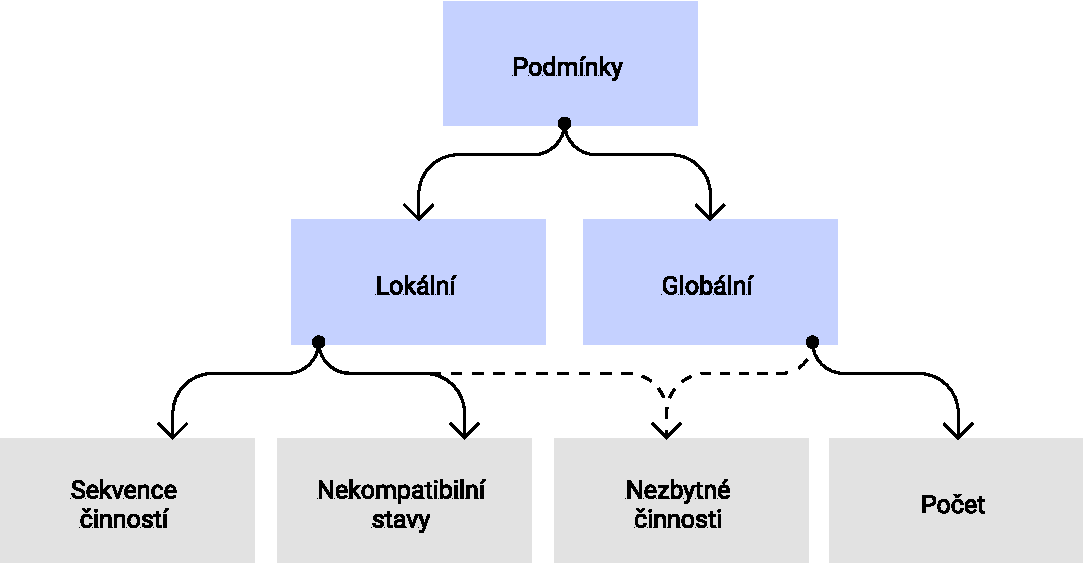
\includegraphics[scale=0.7]{img/constraints.pdf}
	\caption{Rozdělení podmínek dle jejich rozsahu}
	\label{fig:constraints}
\end{figure}

\section{Cílová funkce}
\label{sec:objective}
Cílová funkce je taková funkce, jejíž hodnotu je cílem optimalizovat (minimalizovat nebo maximalizovat). V~případě rozvrhování směn se může jednat o funkce vyjadřující rovnoměrnost obsazení směn, cenu, porušené zbytné podmínky \cite{blochliger2004modeling} či počet kontaktů mezi zaměstnanci (důležitý např. v~případě epidemie) \cite{zucchi2020personnel}.

Například v~případě optimalizace na základě vážených podmínek ji lze formulovat jako rov.~\ref{eq:objective}. Sankce za porušení nemusí být lineární, může jít i~o~konstantu, kvadratickou nebo libovolnou jinou funkci. \cite{kletzander2020solving}
\coloredeq{eq:objective}{
	f(\boldsymbol{x}) = \sum_{s = 1}^n c_s \cdot g_s(\boldsymbol{x}),
}
kde $\boldsymbol{x}$ je dané řešení, $n$ je počet zbytných podmínek, $c_s$ je váha~$s$-té~podmínky (také lze tento údaj chápat jako sankci za její porušení) a $g_s(\boldsymbol{x})$ je počet porušení $s$-té~podmínky v~řešení~$\boldsymbol{x}$. \cite{awadallah2015hybrid}

\section{Matematická interpretace řešení}
Řešení tohoto problému lze interpretovat jako trojrozměrnou binární matici $\boldsymbol{R}$, jejímiž parametry jsou zaměstnanec ($\forall i \in E$), den ($\forall j \in T$) a vypsaná směna ($\forall k \in S$), jednotlivé hodnoty $R_{ijk}$ jsou určeny funkcí \ref{eq:3dmatrix}. \cite{vaclavik2016roster} Takto má smysl řešení interpretovat pouze v~případě, že se obsazují striktně určené sloty pro směny.

\coloredeq{eq:3dmatrix}{
	R_{ijk} =
	\begin{cases}
		1, & \mbox{zaměstnanci $i$ je v den $j$ přiřazena směna $k$,} \\
		0, & \mbox{jinak.}\\
	\end{cases}
}


Příklad toho, jak lze řešení popsané ve funkci~\ref{eq:3dmatrix} interpretovat ve formě tabulky, je v~tab.~\ref{tab:interpretation}.
\begin{table}[h]
	\input{tables/interpretation-example.tex}
	\caption{Interpretace řešení}
	\label{tab:interpretation}
\end{table}


% \section{Rozvrhovací úloha}
% Organizace má množinu zaměstnanců $M$, z~nichž každý zaměstnanec $m \in M$ má určenou množinu činností $Q_m$, které je kvalifikován vykonávat; podmnožině zaměstnanců $E \subseteq M$, $E = \{ 1, 2,~\ldots, e \}$ v~daném období může být rozvrhnuta směna.
%
% % \begin{figure}[h]
% % 	
\includegraphics[scale=0.7]{img/problem-illustration.pdf}
% % 	\caption{Ilustrace problému}
% % 	\label{fig:definition}
% % \end{figure}
%
% Rozvrh se vytváří na období $T = \{1, 2,~\ldots, t \}$ (typicky je toto období rozděleno na dny), v~každém dni jsou vypsány směny $S = \{ 1, 2,~\ldots, s\}$, které jsou charakterizovány např. časovým intervalem nebo požadovanou kvalifikací.
%
% Byla použita některá z~metodik na předpovídání poptávky po personálu (viz podkapitolu \ref{sub:demand}), výsledkem je tabulka (viz např. \ref{tab:demand}), v~buňkách je potřebný počet zaměstnanců v~daném čase (poptávku může určit také rozmezí počtu zaměstnanců nebo to může být relativní veličina).
%
% \begin{table}[h]
% 	\input{tables/demand-tabular.tex}
% 	\caption{Příklad týdenní poptávky}
% 	\label{tab:demand}
% \end{table}
%
% Vstupem mohou být zbytné a nezbytné podmínky a jejich ohodnocení, každý zaměstnanec přitom v jednom čase může být pouze na jednom místě.

% \begin{table}[h]
% 	\begin{tabular}{|@{\makebox[3em][c]{${H}_{\rownumber}$}} |l|c|}
% 	\hline
% 	\multicolumn{1}{|@{\makebox[3em][c]{ID}} | l |}{ Požadavek } & Váha\\
% 	\hline
% 	Všechny směny musí být zaplněny. & 1000 \\
% 	{Každý pracovník může pracovat nejvýše jednu směnu denně.} & 1000 \\
% 	Ranní směna nemůže následovat po noční. & 1000\\
% 	\hline
% 	\end{tabular}
%
% 	\caption{Příklad nezbytných podmínek}
% 	\label{tab:hard}
%
% \end{table}
%
% \begin{table}[h]
% 	\begin{tabular}{@{\makebox[3em][c]{${S}_{\rownumber}$}} |p{0.8\linewidth}|c}
% 	\hline
% 	\multicolumn{1}{@{\makebox[3em][c]{ID}} | l }{ Požadavek } & Váha\\
% 	\hline
% 	\rowcolor{Gray}
% 	{Jsou dodrženy požadavky zaměstnanců na volno.} & 100 \\
% 	{Dvojice zaměstnanců nechce pracovat společně.} & 50 \\
% 	\rowcolor{Gray}
% 	Zaměstnanci mají alespoň dva volné víkendy za sebou & 50 \\
% 	\multicolumn{1}{@{\makebox[3em][c]{$\vdots$ }} | c }{ $\vdots$  } & $\vdots$ \\
% 	\hline
% 	\end{tabular}
%
% 	\caption{Příklad zbytných podmínek}
% 	\label{tab:…
% \end{table}


\section{Deterministické optimalizační metody}

Pro nalezení optimálního řešení mezi všemi možnostmi existuje celá řada metod~–~kromě vyčerpávajícího prohledání celého prostoru může jít o~matematické programování (lineární, kvadratické, nelineární, …).

\subsection{Lineární programování}

Úlohou lineárního programování je nalézt vektor $\boldsymbol{x}^{\ast} \in \mathbb{R}^n$ optimalizující hodnotu cílové funkce mezi všemi vektory, které splňují danou soustavu lineárních rovnic a nerovnic (kterým se zpravidla říká omezující podmínky nebo omezení). \cite{matousek2006linearni}

Celočíselné lineární programování je pro rozvrhování směn vhodné v jed\-no\-du\-chých případech, např.~když jsou pro všechny zaměstnance stanoveny stejné počty po sobě jdoucích pracovních dnů a volna a pro každý den je navíc stanoven minimální počet personálu a cílem je optimalizovat počet zaměstnanců tak, aby byla naplněna poptávka. \cite{satheeshkumar2014linear}

\subsection{Omezení deterministických optimalizačních metod}
Tyto metody obecně můhou přinést optimální výsledky, avšak pro reálné použití je jejich model příliš jednoduchý \cite{burke2004state}, případně špatně škálovatelný.

\section{Heuristika}

Většina stochastických metod vyskytujících se v~literatuře je rozšířením tzv.~metaheuristik, abstraktních metod pro řešení optimalizačních problémů, upravených na problém rozvrhování směn. Narozdíl od deterministických metod řešení není zaručeno, že bude nalezeno optimální řešení, cílem je získat výstup, který je dost dobrý, a to v~dostatečně krátkém čase (co konkrétně to znamená závisí na požadavcích). Neprobíhá tak vyčerpávající prohledávání všech kombinací. \cite{glover2015metaheuristics}

Metody se dají rozdělit do dvou základních skupin -- jedny iterativně rozšiřují částečné řešení, dokud není kompletně dokončeno (lokální vyhledávání), druhé pracují s~platným řešením, které iterativně vylepšují (vylepšovací metaheuristiky). \cite{van2013personnel}

\subsection{Výměna sousedících struktur}
Za účelem vytvoření nebo vylepšení rozvrhu je možné provádět řadu změn, dle \cite{kletzander2020solving} jde například~o:
\begin{itemize}
	\item přidání či odebrání směny,
	\item výměnu směny za jinou,
	\item změnu typu směny,
	\item změnu či vytvoření posloupnosti směn,
	\item výměnu směn mezi zaměstnanci,
	\item výměnu směn zaměstnance,
	\item zkrácení směny.
\end{itemize}


\subsection{Tabu search}
Základem tabu search je existence dvou druhů paměti – krátkodobé (obsahuje naposledy navštívená řešení) a dlouhodobé (obsahuje frekvenci návštěv). \cite{liang2020optimization} Vytváření a vylepšování řešení probíhá způsobem dle obr.~\ref{fig:tabusearch} tak, aby byly splněny podmínky. Prohledávání prostoru probíhá v~blízkém sousedství řešení, které je omezeno tak, aby se řešení nezacyklilo (jsou určeny zapovězené kroky -- tabu -- v~krátkodobé paměti, aby nebyla procházena stále stejná, dále již cílovou funkci nezlepšující řešení -- co je tabu, lze použít pouze tehdy, když řešení splňuje aspirační kritéria).  \cite{glover1990tabu}

\begin{figure}[h]
	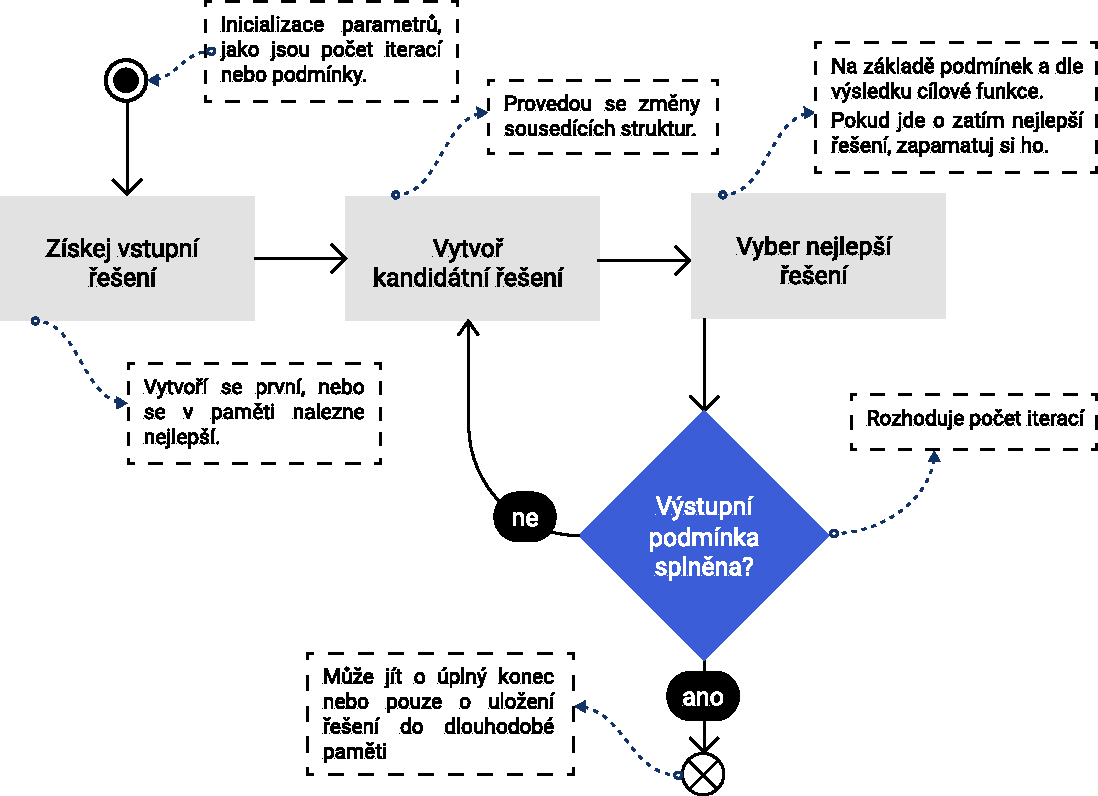
\includegraphics[scale=0.7]{img/tabu-search.pdf}
	\caption{Metaheuristika tabu search}
	\label{fig:tabusearch}
\end{figure}

% Ve verzi popsané v~\cite{ramli2020tabu} se rozeznávají dvě skupiny zaměstnanc dle úrovně zkušeností (konkrétně se jedná o~rozvrhování zdravotních sester) – seniorní a juniorní.
 Algoritmus začíná inicializací řešení částečně náhodným způsobem tak, aby řešení neporušovalo nezbytné podmínky. Vylepšování referenčního řešení probíhá pomocí výměny sousedících struktur (dle podmínek např.~výměna posloupnosti směn mezi dvěma zaměstnanci). \cite{ramli2020tabu}

% Prvním krokem je výběr tří po sobě jdoucích dnů, kdy má zaměstnanec noční směnu, po nichž následují dva dny, kdy noční směnu nemá, dále se rozřadí volné dny a denní směny (viz~obr.~\ref{fig:tabusearchfirst}). Optimalizace tak probíhá na řešení, které neporušuje žádné nezbytné podmínky (např.~ranní směna nenásleduje po noční, zaměstnanec má nejvýše $k$ po sobě jdoucích pracovních dnů a alespoň jeden den volna týdně, počet zaměstnanců na směně je alespoň $n$). Hlavní cíle jsou rovnoměrné rozložení zkušených a nezkušených zaměstnanců, minimalizace porušení podmínek u jednotlivých zaměstnanců a minimalizace porušení podmínek v~rámci jednotlivých dní.

% \begin{figure}[h]
% 	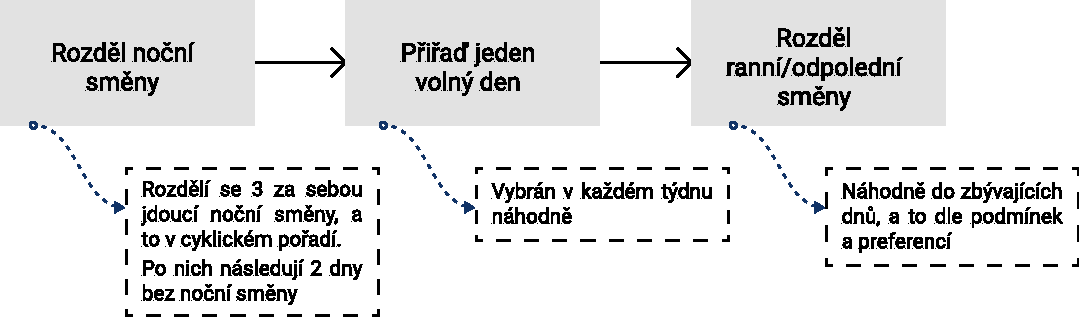
\includegraphics[scale=0.7]{img/tabu-search-first-step.pdf}
% 	\caption{Inicializace řešení}
% 	\label{fig:tabusearchfirst}
% \end{figure}

\subsection{Genetický algoritmus}

Genetický algoritmus je metaheuristika inspirovaná genetikou~--~používají se operace nazvané selekce chromozomů, křížení a mutace.

Narozdíl od tabu search se v~genetickém algoritmu prohledává větší množina řešení~–~začíná se s~počáteční populací řešení, v~níž se selektují nejlepší řešení, která se dále mezi sebou kříží~(kombinace náhodných částí), případně nahodile mutují. Algoritmus končí, pokud řešení konverguje~–~už se dlouhou dobu nepodařilo ho vylepšit. \cite{mallawaarachchi2017introduction}

Tento přístup lze aplikovat na rozvrhování směn například tak, že se jako chromozom kóduje kombinace dne, směny a zaměstnance. \cite{maenhout2011evolutionary}


\chapter{Analýza systému}

%Cílem této práce je navrhnout mobilní aplikaci pro plánování lidských zdrojů, obzvláště rozvrhování směn. Bude se tak jednat o aplikaci, která bude sloužit pro zjednodušení interních procesů v~rámci nějaké firmy, půjde o~minimalistický informační systém pro zaměstnance a zaměstnavatele. Pro účely identifikace požadavků bude v~této kapitole vytvořen předpoklad o~cílové skupině organizací, které by mohly tento software nasadit, jaká je jejich současná situace a co by jim mělo toto softwarové řešení poskytnout. Rovněž budou z~uživatelského pohledu popsána již existující softwarová řešení, která jsou pro dané situace určena.

\section{Cílová skupina}
Aby bylo možné stanovit požadavky na aplikaci, byl vytvořen předpoklad o~cílové skupině pro tento systém. Jedná se o~menší firmu (případně malý tým v~rámci větší firmy) o~10 až 20 zaměstnancích, která podniká v~nekritickém vícesměnném provozu (např.~jedna pobočka řetězce rychlého občerstvení, restaurace nebo obchod). Firma zaměstnává jak pracovníky s~pracovní smlouvou, tak brigádníky na DPP/DPČ. Vzhledem k~tomu řeší problém, jak rozvrhovat směny, stávající způsob je z~pohledu vedení firmy i samotných zaměstnanců neefektivní například z následujících důvodů:
\begin{itemize}
	\item brigádníci si musí směny domlouvat osobně,
	\item rozvrh je pověšen pouze na nástěnce,
	\item rozvrh se sestavuje manuálně,
	\item nedodržuje se týdenní pracovní doba,
	\item rozvrh je sestaven dle osobních preferencí vedoucího.
\end{itemize}


\section{Požadavky z~pohledu organizace}

Následující požadavky definují, jaké základní funkce by měl tento systém mít, a to především z~pohledu organizace, která by jej využívala (jedná se o~požadavky s~vysokou mírou abstrakce). Vychází se z~představy popsané výše, tedy že tento software je určen pro nasazení ve firmě, která momentálně není schopna efektivně připravovat rozvrhy směn a chtěla by ušetřit čas a zdroje, které na sestavení rozvrhu vynakládá.

\begin{enumerate}[label=\textbf{B\arabic*.}]
	\item Systém umožní distribuci rozvrhů směn k~zaměstnancům.
	\item Systém umožní zápis zaměstnance na~DPP/DPČ na směnu.
	\item Systém vytvoří rozvrh směn na základě požadavků organizace.
	\item Systém bude automatizovat dohled nad dodržováním legislativy.
\end{enumerate}

\section{Doménový model}

V diagramu \ref{fig:domainmodel} je zadefinován předpokládaný doménový model firem cílové skupiny, jde o~znázornění skutečnosti, že ve firmě pracují zaměstnanci, kteří mají smlouvy a kterým jsou do jejich rozvrhu přiřazeny směny.

\begin{figure}[h]
	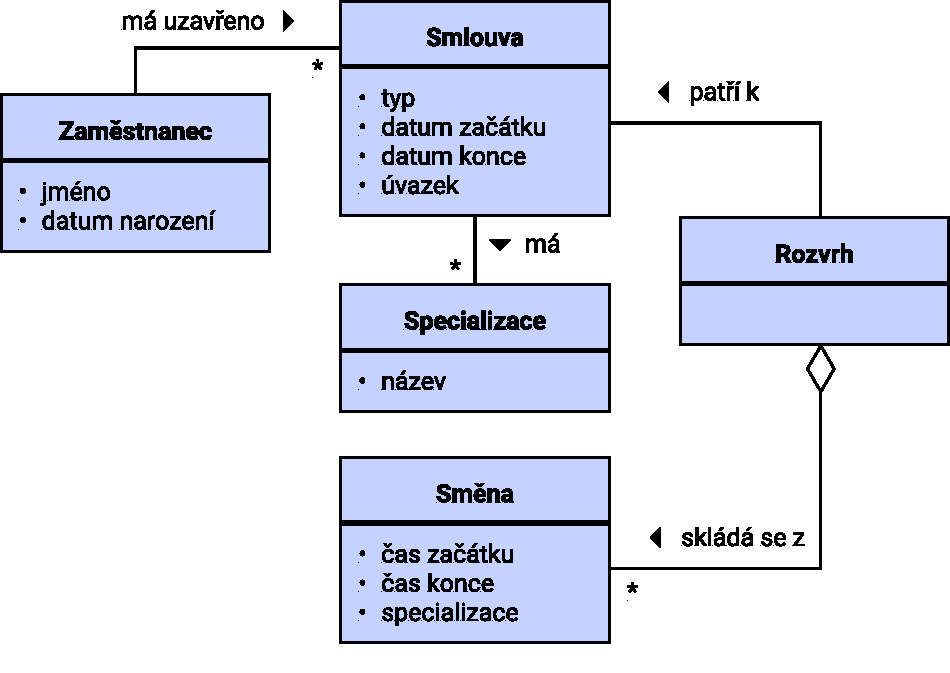
\includegraphics[scale=0.7]{img/domain-model.pdf}
	\caption{Doménový model}
	\label{fig:domainmodel}
\end{figure}

\section{Analýza existujících řešení}
\label{sec:existing}
Tato podkapitola bude věnována popisu již existujících nástrojů pro plánování lidských zdrojů. Jedná se o komerční software, který byl otestován v~demoverzi, vzhledem k~tématu této práce byly hlavními sledovanými aspekty mobilní aplikace pro zaměstnance a~způsob rozvrhování směn.

Tyto systémy lze zařadit do kategorie tzv.~informačních systémů pro řízení lidských zdrojů, jejichž úkolem je obecně jak automatizovat, tak podporovat strategické rozhodování na základě dat. \cite{kovach2002administrative}

Byly vybrány informační systémy pro plánování lidských zdrojů, které alespoň částečně odpovídají uvedeným požadavkům z~pohledu organizací~–~podporují samoobslužné sestavování rozvrhů a případně i~tvorbu rozvrhů nějakým způsobem automatizují.

\subsection{Tamigo}
Aplikace Tamigo\footnote{\url{https://www.tamigo.cz/}} je komplexní aplikace pro plánování lidských zdrojů, je určena pro použití v~pohostinství, maloobchodě, zdravotnictví aj. \cite{tamigo2020reseni}

Aplikace je organizacím nabízena v~několika variantách, které jsou zpop\-lat\-ně\-ny podle množství podporovaných funkcí (jedná se např. o~rozpisy směn všech zaměstnanců, výkazy práce, správu absencí, správu mezd smluv zaměstnanců, evidenci příchodů a odchodů) a počtu zapojených zaměstnanců. Mezi součásti tohoto produktu patří webové rozhraní i mobilní aplikace (přestože jde o nativní aplikaci, v~testované verzi funguje pouze v~případě, že je uživatel online, jinak padá). Uživatelské role jsou v~tomto systému Administrátor, Manažer a Zaměstnanec.

Systém umožňuje manažerům vytvářet rozvrh, částečně je tento proces manuální, částečně lze rozvrh vygenerovat na základě šablon, které si uživatel předem připraví (např. obvyklá pracovní doba pro jednotlivé zaměstnance).

Za\-měst\-na\-nec si může aktualizovat osobní data, zobrazit osobní rozvrh směn, žádat o dovolenou a sledovat stav jejího čerpání, zobrazit výkaz práce pro výplatní období, aj.

\subsection{Tanda}
Na podobném principu jako aplikace Tamigo pracuje i~aplikace Tanda\footnote{\url{https://www.tanda.co/}}. Automatické rozvrhování funguje na principu šablon -- rozvrh se tedy vytvoří jednou a následně se opětovně používá \cite{tanda2020rosters}.

I tento systém má jak webové, tak mobilní rozhraní, obojí pro zaměstnance i vedoucí. Mobilní rozhraní opět nepodporuje ani čtení dat v~případě, že je uživatel offline.

\subsection{When I Work}
Aplikace When I Work\footnote{\url{https://wheniwork.com}} má opět webové i mobilní rozhraní. Rozvrhování zde opět funguje manuálně nebo na základě šablon, aplikace v~placené Pro verzi \cite{wheinwork2020pricing} však podporuje i automatické přiřazení volných směn k~vhodným zaměstnancům (v~potaz při rozvrhování bere pracovní pozici, již existující směny, požadavky na volno a další filtry). \cite{wheinwork2020employee} Mobilní aplikace umožňuje zaměstnancům zadat, jakou pracovní dobu preferují nebo kdy jsou naopak nedostupní. Ani tato aplikace nefunguje v~offline režimu.

\subsection{Shrnutí}
Vyzkoušené informační systémy se v~principu příliš neliší a nabízejí podobné základní prvky (mobilní a webové rozhraní; uživatelské role; komplexní správa mezd, docházky, rozvrhů). Společné mají i to, že žádná z~aplikací neimplementuje ani částečný offline režim, což může být pro uživatele v~některých situacích nepříjemné (lze ale předpokládat, že mobilní aplikace nebyla tvůrci považována za prioritní v~porovnání s~webovým rozhraním). Liší se však způsobem, jakým rozvrhují směny -- největší automatizaci zde poskytuje aplikace When I Work. Dalším rozdílem je uživatelská přívětivost, její hodnocení by však bylo spíše subjektivní.

Alternativou systémů, které přímo odpovídají požadavkům, mohou být komplexnější ERP systémy a jejich modul pro plánování lidských zdrojů.

\section{Požadavky na systém}
Na základě požadavků ze strany organizace a~po otestování podobných aplikací byly stanoveny požadavky na funkce nového systému, které byly rozděleny do několika kategorií podle cílového uživatele. Při implementaci systému na plánování směn je žádoucí, aby byl dohled nad dodržováním pracovněprávních předpisů (především těch, které uvádějí kvantitativní údaje), automatizován, proto jsou rovněž uvedeny požadavky vyplývající z~analýzy legislativy (viz podkapitolu \ref{section:legislativa}).

\subsection{Uživatelé}
\begin{enumerate}[label=\textbf{U\arabic*.}]
		\item Systém bude personalizovaný podle potřeb daného uživatele.
\end{enumerate}

\subsection{Zaměstnanci}
\begin{enumerate}[label=\textbf{Z\arabic*.}]
		\item Systém umožní zaměstnancům náhled do jejich rozvrhu.
		\item Systém umožní zaměstnancům na DPP/DPČ zápis na směnu.
\end{enumerate}

\subsection{Organizace}
\begin{enumerate}[label=\textbf{O\arabic*.}]
	\item Systém umožní registraci nových organizací.
	\item Systém umožní přidávání nových zaměstnanců.
	\item Systém umožní automatické přiřazení směn.
	\item Systém umožní plánování směn na následující týdny.
	\item Systém umožní náhled na rozvrh zaměstnanců.
\end{enumerate}

\subsection{Legislativa}
\begin{enumerate}[label=\textbf{L\arabic*.}]
		\item Systém umožní náhled do osobního rozvrhu nejméně 2 týdny předem.
		\item Systém umožní zaměstnancům na dohodu o~provedení práce odpracovat nejvýše 300~hodin v~kalendářním roce.
		\item Systém umožní zaměstnancům na dohodu o~pracovní činnosti odpracovat nejvýše 20~hodin týdně v~průměru 52 týdnů.
		\item Systém rozvrhne směny s~ohledem na 40hodinovou týdenní pracovní dobu a úvazky jednotlivých zaměstnanců.
\end{enumerate}

\section{Aktéři, uživatelské role}
Jedním z~hlavních cílů systému na plánování směn je informovat každého zaměstnance o jeho směnách, proto se jeví vhodnou personalizace, které se docílí s~pomocí uživatelských účtů. Vstupní operací bude přihlášení -- z~toho vyplývá nezbytnost existence role přihlášeného a nepřihlášeného uživatele.

Pro roli přihlášeného uživatele je nutné další rozšíření, konkrétně na zaměstnance a roli, kterou má v~rámci tohoto systému za\-měst\-na\-va\-tel či jím pověřená osoba (vedoucí), která má zodpovědnost za rozvrhování pracovní doby a která by měla mít komplexní přehled o rozpisu i možnost do něj zasáhnout.

Jednotliví zaměstnanci pak v~systému mohou být různými aktéry, především na základě pracovněprávního vztahu (tj. zaměstnanec v pracovním poměru, zaměstnanec na dohodu o provedení práce a zaměstnanec na dohodu o pracovní činnosti), viz obr.~\ref{fig:userroles}. Důvodem je, že aktéři budou moci provádět specifické operace a systém s~nimi bude interagovat odlišně. Rozhodujícím faktorem není to, zda má zaměstnanec plný nebo zkrácený úvazek, v obou případech platí stejné podmínky a liší se jen týdenní pracovní doba, stejně tak nezáleží na tom, zda je zaměstnanec nezletilý.

\begin{figure}[h]
	\input{img/actors.pdf_tex}
	\caption{Diagram aktérů}
	\label{fig:userroles}
\end{figure}

\newpage
\section{Uživatelské příběhy}\label{uc-analysis}

Pro analýzu systému z~pohledu uživatelské interakce byl zvolen neformální způsob inspirovaný uživatelskými příběhy (user stories), hlavní výhodou je využití běžného jazyka. Přehled uživatelských příběhu ve zjednodušené podobě je na obr.~\ref{fig:user-stories}, jejich podrobnější mapa je součástí přílohy \ref{sec:user-story}. Interakci uživatele a systému se rovněž věnuje příloha \ref{sec:ui}, která obsahuje náčrty uživatelského rozhraní a jejich popis.

\begin{figure}[h!]
	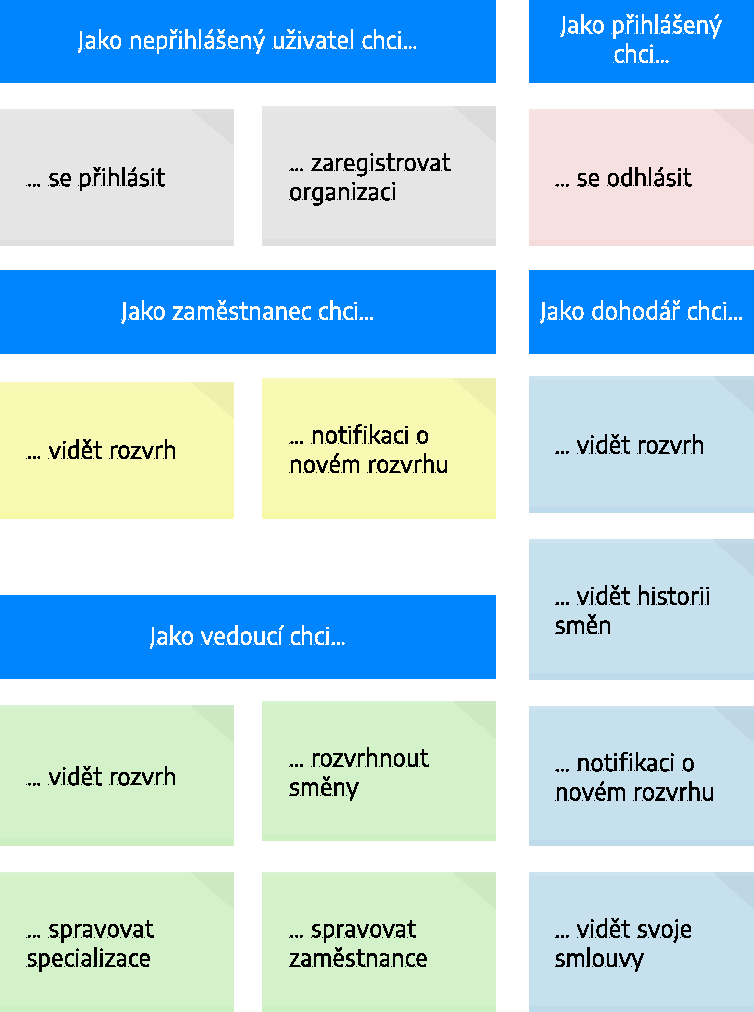
\includegraphics[scale=0.7]{user-stories.pdf}
	\caption{Zjednodušený storyboard}
	\label{fig:user-stories}
\end{figure}

\newpage

\part{Praktická část, implementace}

\chapter{Výběr technologií}
%Při výběru technologií pro tento projekt hrály kromě samotných požadavků na tuto aplikaci roli i zkušenosti a preference autorky, konkrétní výběr byl tedy zkreslen i subjektivním hlediskem.

\section{Technologie pro uživatelské rozhraní}

V~případě, že by byla aplikace určena k~nasazení v~produkčním prostředí, připadaly by v~úvahu nejméně dva přístupy -- mobilní nebo webová aplikace.

\begin{figure}[h!]
	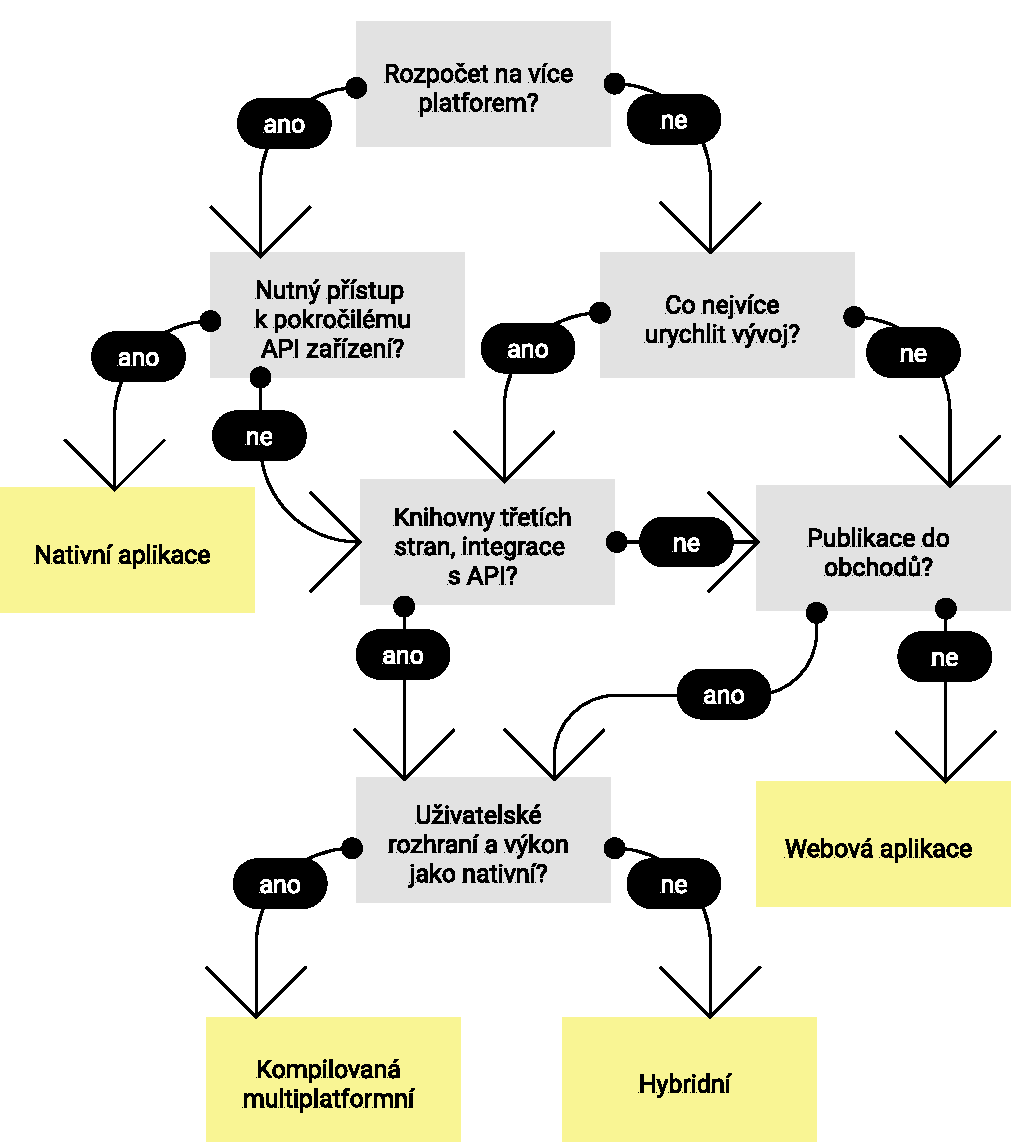
\includegraphics[scale=0.7]{img/app-decision-tree.pdf}
	\caption{Rozhodovací strom pro vývoj na mobilní zařízení}
	\label{appdecisiontree}
\end{figure}

\subsection{Webová aplikace}
Pro použití webové aplikace hovoří fakt, že je není třeba žádným způsobem instalovat a stačí prosté zadání adresy do internetového prohlížeče, z~podstaty věci je multiplatformní, lze ji zobrazit jak na počítači, tak na mobilním zařízení, jedná-li se o responzivní aplikaci, může být i~její použití na mobilním zařízení uživatelsky přívětivé. Nevýhodami jsou omezené možnosti při implementace offline režimu, i to, že z hlediska rychlosti se nativním mobilním aplikacím nevyrovnají. \cite{stevens2018what}

\subsection{Mobilní aplikace}

Vyplývá-li podpora mobilní platformy z~požadavků, ilustruje další rozhodování o~způsobu implementace strom na obrázku \ref{appdecisiontree} (vychází z~\cite{matyunina2020native}), především ale záleží na prioritách toho, kdo danou aplikaci chce uvádět na trh.

Oproti responzivnímu webu mají nativní aplikace výhodu, že mohou jednoduše přistupovat k API, které poskytuje zařízení, na kterém jsou nainstalované, tedy mohou snadno získat přístup k fotoaparátu či poloze zařízení; také lze na zařízení jednoduše přijímat notifikace, i když je aplikace na pozadí. Nativní aplikace mohou být vhodné i pro použití v offline režimu, aplikace může mít lokální databázi.

Nevýhodou pro uživatele je, že se musí instalovat na zařízení. S~tím souvisí i o~něco složitější způsob distribuce -- v~případě, že je možné zveřejnit aplikaci v~obchodech (Google Play, AppStore), musí projít schvalovacím procesem, což může trvat několik dní a nemusí být vždy úspěšné, např. v~případě, že aplikace obsahuje nevhodný obsah, narušuje něčí autorská práva nebo nevhodným způsobem zpracovává osobní údaje uživatelů. Je třeba uvádět, jaká oprávnění pro přístup ke mobilním API (SMS, kontakty, poloha, soubory, aj.) aplikace požaduje. \cite{google2021policy}.

Při výběru konkrétního způsobu implementace mobilní aplikace pak existuje několik dalších rozhodovacích situací, především~výběr podporované platformy.

\subsubsection{Platforma}
Na trhu s~chytrými mobilními zařízeními jsou dvě dominantní platformy, Android (podíl na trhu celosvětově 72~\%) a iOS (podíl na trhu 27,5~\%) \cite{statcounter2021mobile}. Nevýhodou rozšířenějšího Androidu oproti iOS je fragmentace, tzn. existence velké řady různých zařízení, která je třeba podporovat. Pro účely této práce bude podporována pouze platforma Android.


\subsubsection{Způsob vývoje}

Je-li nezbytné podporovat více platforem, je možné vyvinout aplikaci multiplatformně, hybridně, případně pro každou platformu zvlášť.

\paragraph{Multiplatformní vývoj}
Multiplatformní vývoj umožňuje nasazení jedné aplikace na více platformách, kód pro všechny platformy je sdílený, jádro aplikace tedy není třeba duplikovat, což je jejich nespornou výhodou, navíc to může i snížit náklady na vývoj.

Problémem je přístup k~aplikačnímu rozhraní a hardwaru daného zařízení, omezené možnosti při používání knihoven specifických pro platformu nebo složitější vývoj uživatelského rozhraní tak, aby odpovídalo konvencím pro všechny platformy. \cite{manchanda2020where}   Používají se frameworky jako Flutter (jazyk Dart), React Native (JavaScript) nebo Xamarin (C\#).

\paragraph{Vývoj pro danou platformu}
V~případě vývoje na jednu platformu je možné používat všechny součásti zařízení naplno. Co se přístupu k hardwaru, výkonu a uživatelské přívětivosti týče, mají nativní aplikace nad multiplatformními jasnou převahu, jejich vývoj je však dražší. \cite{dennis2018native}

\paragraph{Hybridní vývoj}
Hybridní aplikace jsou kombinací webu a nativní mobilní aplikace – použijí se standardní technologie pro vývoj webu (HTML + CSS + JavaScript), toto se obalí do nativní aplikace, v~níž běží webový prohlížeč. Jejich největší výhodou je cena, rychlost vývoje a jednodušší správa. Stinnou stránkou tohoto přístupu je menší uživatelská přívětivost, omezený přístup k~API zařízení nebo nižší výkon v~porovnání s~plně nativní aplikací. \cite{design2020ultimate}


\subsubsection{Programovací jazyk}
Pro nativní vývoj na platformu Android lze vybrat nejméně ze tří možností, a to C/C++, Javy a Kotlinu. Toto rozhodování může v~této době u~nových projektů probíhat spíše pouze v teoretické rovině, neboť oficiální podporu ze strany Googlu má nejmodernější jazyk Kotlin.

Mezi hlavní výhody Kotlinu oproti jiným variantám patří null-safety (bezpečné volání na objektech, které mohou nabývat hodnotu \texttt{null}), coroutines (odlehčená verze vláken pro asynchronní operace) nebo Kotlin Extensions (knihovny nejrůznějších funkcí usnadňující vývoj obecně i specificky pro Android). \cite{android2021kotlin}

Obdobné rozhodování může probíhat i~v~případě platformy iOS, pro kterou se nabízí použití Swiftu nebo starého jazyka Objective-C. Ze strany Applu je doporučena modernější varianta (Swift), protože aplikace jsou rychlejší a vývoj snazší.

\subsubsection{Architektonický vzor}
Standardním architektonickým vzorem používaným při vývoji Android aplikací je MVVM. \cite{android2020guide}. Aplikace má tři vrstvy, které spolu komunikují způsobem naznačeným na obr.~\ref{fig:mvvm}. Hlavním cílem je oddělit prezentační vrstvu od business logiky.  \cite{shekhar2020mvvm}

\begin{figure}[h!]
	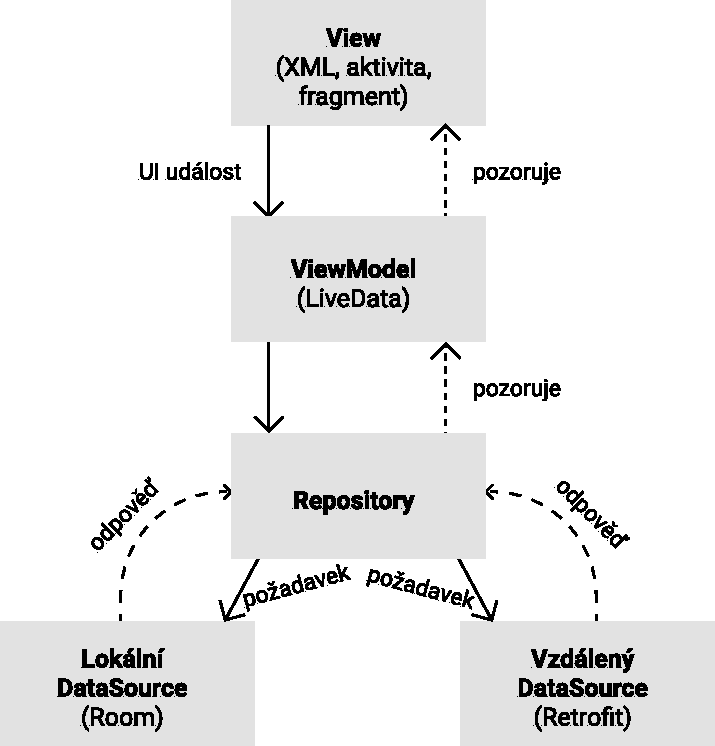
\includegraphics[scale=0.7]{img/mvvm-architecture.pdf}
	\caption{Komunikace mezi vrstvami v~MVVM}
	\label{fig:mvvm}
\end{figure}

MVVM vychází ze staršího architektonického vzoru MVP\footnote{Model-View-Presenter}, Presenter je podobný jako ViewModel, hlavním rozdílem je, že Presenter si drží referenci na View (relace mezi View a Presenterem je 1:1) a řídí, kdy se má View aktualizovat, kdežto ViewModel neví, jaký View ho pozoruje a relace mezi View a ViewModelem je 1:$n$. \cite{vogel2017android} Nadstavbou nad MVVM je tzv.~Clean Architecture, která zaručuje ještě větší oddělení prezentační vrstvy a business logiky (Android aplikace se rozděluje do více modulů, nejčastěji nazvaných Presentation, Domain a Data). \cite{jain2019kotlin}

% \begin{figure}[h!]
% 	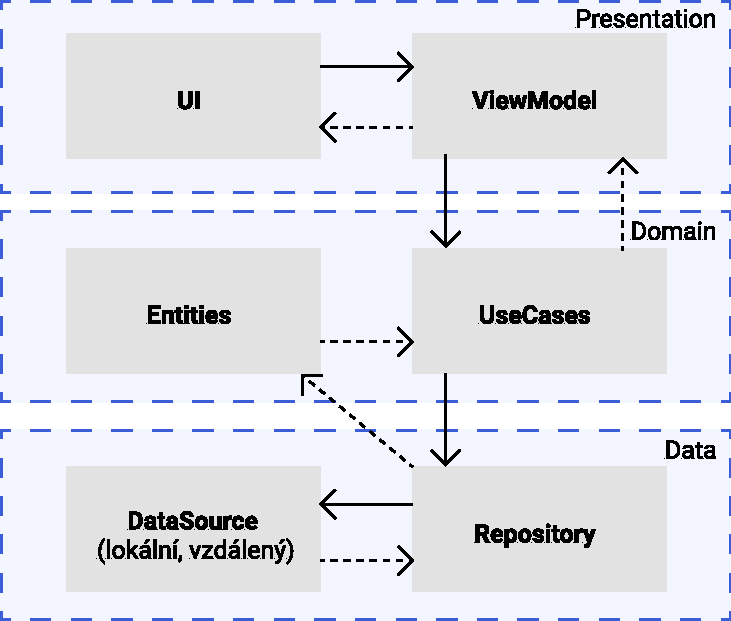
\includegraphics[scale=0.7]{img/clean-architecture.pdf}
% 	\caption{Clean Architecture}
% 	\label{fig:clean-architecture}
% \end{figure}

Vzhledem k~předpokládané velikosti projektu byl zvolen doporučený architektonický vzor MVVM.

\subsection{Shrnutí}

Jako nejvhodnější by se v~případě produkčního nasazení této aplikace jevilo zkombinovat oba přístupy, tedy mít uživatelské rozhraní jak ve formě webové aplikaci, tak mít i podpůrnou mobilní aplikaci. Tento přístup byl také zvolen v případě většiny podobných řešení (viz podkapitolu \ref{sec:existing}). Zde byla implementována pouze jedna část, a to mobilní aplikace, neboť důraz byl kladen především na pohodlí zaměstnanců, kteří chtějí mít svůj rozvrh po ruce co nejrychleji. %Pokud by naopak bylo prioritou vytvořit rozhraní přívětivé pro zobrazení přehledu o celkovém rozvrhu všech zaměstnanců, které vyžaduje větší rozlišení obrazovky, dávalo by větší smysl implementovat nejprve webové rozhraní.

Mobilní aplikace bude vyvinuta jako nativní Android aplikace, tento výběr je zkreslen zkušenostmi autorky, v~produkčním prostředí by bylo žádoucí uživatele iOS nediskriminovat a aplikaci jim také nabídnout, z~tohoto důvodu by bylo vhodné zvážit použití nějakého multiplatformního frameworku, rozhodující by byly plány na budoucí vývoj, případně i~finance. Pro vývoj se použije programovací jazyk Kotlin, protože se jedná o moderní programovací jazyk, který je pro vývoj na danou platformu nejvhodnější. Aplikace bude navržena dle zásad architektonického vzoru Model-View-ViewModel.


\section{Backendová technologie}

\subsection{Webový framework}

Webové frameworky, tj. knihovny zdrojových kódů připravené pro tvorbu webů (především jejich serverové strany), se standardně používají pro zjednodušení vývoje a nasazení aplikací. Ať už jsou napsány v~libovolném programovacím jazyce (může jít např.~o~PHP, Javu, Ruby nebo Python), standardními součástmi jsou perzistence dat, autentizace uživatelů, správa session nebo šablony pro uživatelské rozhraní. Společnou mají také podporu pro architektonický vzor MVC. \cite{docforge2014web}

Z~množství variant, které se nabízejí, byl zvolen framework Ruby on Rails (v~jazyce Ruby), a to především z~důvodu jeho filosofie Don't Repeat Yourself (kód by měl být znovupoužitelný, bez zbytečného opakování) a Convention Over Configuration (webová aplikace je nakonfigurována dle konvencí, a vývojář tak nemusí trávit čas psaním konfiguračních souborů) \cite{rails2020}, která slibuje výrazné usnadnění vývoje.

\subsection{Aplikační rozhraní}

Pro komunikaci s~dalšími aplikacemi (zde především pro komunikaci klienta se serverem) musí aplikace vnějšku poskytnout své aplikační rozhraní. Za tímto účelem existuje několik možností, které jsou vhodné pro různé případy (např.~REST, SOAP, GraphQL, gRPC). Tyto způsoby implementace se mohou od sebe odlišovat formátem přenosu (binární, textový) nebo protokolem (HTTP i~jiné).

Pro účely tohoto projektu se jako optimální varianta jeví použití REST API, a to vzhledem k~velmi dobré podpoře ze strany webového frameworku bez nutnosti rozšiřování o~další knihovny (konkrétně Ruby on Rails podporují vytváření cest na základě konvencí – pokud tak controller definuje metodu \texttt{update}, automaticky se vytvoří endpoint \texttt{PUT/PATCH /resources/:id}, případně lze cesty definovat v~souboru \texttt{config/routes.rb} a provolat tak libovolnou akci v~libovolném controlleru).

V některých případech by bylo vhodnější použít pro komunikaci jiný prostředek (především v~případě volání výpočtů na serveru), např.~RPC (gRPC, XML-RPC, JSON-RPC či jinou konkrétní implementaci), neboť zde nedochází k~přenosu zdrojů, ale pouze k~výpočtům na vzdáleném serveru (provolávání akcí). \cite{sturgeon2016understanding} Toto by ale vytvořilo problémy při nasazení aplikace na PaaS službách (např. Heroku) \cite{lisitsky2018does}, proto bylo zvoleno řešení, které sice není z~hlediska architektury tou nejlepší volbou, ale jeho  použití je flexibilnější.

\subsection{Databáze}

Rozhodování ohledně použité databáze se může týkat způsobu uložení dat (relační nebo NoSQL) a samotného DBMS (systém správy báze dat). Je třeba se rozhodnout, zda v~projektu bude použita relační či NoSQL databáze. Relační databáze přitom jsou vhodné na ukládání dat se statickou strukturou, NoSQL databáze mohou být flexibilnější, co se ukládání dat týče.  \cite{geeks2020difference}

Pro účely tohoto projektu byla zvolena relační databáze, a to z~důvodu předem určené struktury dat a taktéž proto, že jde o technologii, která má dobrou podporu, a to i ze strany webových frameworků. Upřednostněna tedy byla známá technologie. Jako konkrétní DBMS byl zvolen Postgres.


\subsection{Shrnutí}

Aplikace bude vyvinuta ve webovém frameworku Ruby on Rails, a to vzhledem k~tomu, že jde o~rozšířený framework, který slibuje jednoduchou konfiguraci. Z~volby frameworku vyplývá použit architektonického vzoru MVC. S~vnějškem bude tato aplikace komunikovat prostřednictvím REST API vzhledem k~jednoduché implementaci a silné podpoře pro jeho využití. Použita bude relační databáze, konkrétně Postgres.

\section{Požadavky na kvalitu software}

Z~rozhodování v~této kapitole vyplynuly následující požadavky na kvalitu software:

\begin{enumerate}[label=\textbf{S\arabic*.}]
	\item Bude vyvinuta nativní Android aplikace v~jazyce Kotlin.
	\item Backend bude vyvinut ve webovém frameworku Ruby on Rails.
	\item Mobilní aplikace bude se serverem komunikovat přes jeho REST API.
	\item Bude použita databáze Postgres.
\end{enumerate}

\chapter{Návrh vlastního algoritmu}

\section{Požadavky na rozvrh}

Z~hlediska klasifikace uvedené v~podkapitole~\ref{sec:clasif} půjde o neperiodický rozvrh s~flexibilními parametry, cílem bude spíše rozhodnout než optimalizovat. Nezbytné podmínky budou dány legislativními požadavky na rozvrh směn; rozvrh bude sestaven nejméně na týden. Předpokládá se, že jiné směny budou dále rozvrhnuty jiným způsobem. Cílem je netvořit zbytečné překážky v~zaměstnání a rozvrhnout práci všem.

Konkrétní požadavky byly stanoveny následovně:
\begin{enumerate}
	\item Algoritmus rozvrhne směny na jeden týden.
	\item Algoritmus rozvrhne směny v~celém dni na základě poptávky.
	\item Algoritmus rozdělí směny mezi zaměstnance v~pracovním poměru.
	\item Algoritmus rozdělí směny mezi všechny zaměstnance, kteří mají v~daném týdnu pracovat.
	\item Algoritmus vezme v~potaz legislativní požadavky.
\end{enumerate}

\section{Tvorba směn a poptávky}\label{sub:demand}
Při rozvrhování se pro zjednodušení předpokládá, že v každém týdnu budou vypsány směny pravidelným způsobem, to znamená, že všechny budou stejně dlouhé a budou každý den v~týdnu začínat ve stejnou dobu, a budou v rámci jednoho pracovního dne rozloženy pravidelně dle počtu směn (pro realističtější modelování situace existuje možnost některé směny z rozvrhu vyjmout). Půjde tak flexibilně stanovit parametry rozvrhování, konkrétně celkovou pracovní dobu, délku jedné směny, délku přestávky a počet směn v jednom dni. Bude také možné naplánovat směny probíhající přes noc, případně i~24hodinový provoz (pak bude třeba stanovit začátek jedné ze směn, aby bylo možné jejich rovnoměrné rozdělení). Pro každou jednotlivou směnu lze dále určit její prioritu (číslo mezi 0~a~5).

\section{Podmínky}
Obdobně jako v~podkapitole \ref{sec:constraints} se podmínky dají rozdělit do dvou skupin (nezbytné a zbytné).

\subsection{Nezbytné podmínky}
Pro určení nezbytných podmínek byly využity poznatky z~oblasti legislativy (viz podkapitolu \ref{section:legislativa}), především maximální délka směny, minimální přestávka mezi koncem jedné směny a začátkem další, týdenní pracovní doba, dále také určení specializace.

Rozvhování probíhá v~transakci a tyto podmínky jsou vyhodnocovány na úrovni modelů, v~případě, že budou porušeny, bude vyvolána výjimka, dojde k~rollbacku a zahození celého rozvrhu.

Konkrétně se jedná o následující podmínky:

\begin{enumerate}
	\item Zaměstnanec v~celém týdnu odpracuje nejvýše počet hodin úměrný svému úvazku.
	\item Mezi koncem jedné směny a začátkem další bude nejméně 12hodinová přestávka.
	\item Zaměstnanec může být přiřazen pouze na směnu, která nemá žádnou specializaci nebo má stejnou specializaci jako zaměstnanec.
	\item Zaměstnanec může být v jednu chvíli pouze na jedné směně, směny se nesmějí překrývat.
\end{enumerate}

\subsection{Zbytné podmínky a cílová funkce}
Byly zvoleny čtyři zbytné podmínky (obsazení všech směn, obsazení směn úměrně poptávce, obsazení specializovaných směn, více volna v~kuse). Pro každou z~nich byl zvolen způsob, jak se bude počítat cílová funkce, dále byl stanoven pokud možno co nejjednodušší způsob, jak optimalizovat hodnotu cílové funkce.

Cílová funkce je stanovena obdobně jako v~podkapitole \ref{sec:objective} – jde o~součet vážených porušení zbytných podmínek (sankce za porušení je lineární).

\subsection{Obsazení všech směn}

Smyslem této podmínky je určit, zda v~každou chvíli bude na pracovišti alespoň jeden zaměstnanec. Vyhodnocení probíhá tak, že se naleznou všechny směny, které nemá do svého rozvrhu zapsán žádný zaměstnanec. Výsledkem cílové funkce je počet neobsazených směn násobený sankcí.

\subsection{Obsazení směn úměrně poptávce}
Jak již bylo uvedeno v podkapitole \ref{sub:demand}, každá ze směn může mít určenou svou prioritu. Penalizována je odchylka od požadovaného obsazení $\texttt{D[i]}$ pro $\texttt{i} = \mbox{priorita dané směny}$ v~souhrnném rozvrhu (jde tak o~globální podmínku).


\subsubsection{Rozložení poptávky}
Pro účely rozložení poptávky mezi směny s~různou prioritou byl navržen následující postup: nejprve se spočítá průměrná priorita (\texttt{avg\_priority}) ze všech směn v~daném období a průměrný počet zaměstnanců na jednu směnu (\texttt{avg\_assignments}, počet přiřazení na směnu dělený počtem směn).

Z těchto údajů se vypočítá požadovaný počet zaměstnanců na směně o~střední prioritě (\texttt{medium\_demand = 3}). \texttt{const} je nějaká konstanta, která ovlivňuje rozložení poptávky (viz tab.~\ref{tab:demandfactor}). Hodnota konstanty by měla být alespoň \texttt{medium\_demand}, aby poptávka byla kladné číslo. S~výsledkem rov.~\ref{eq:d3} a \ref{eq:di} se pracuje v zaokrouhlené formě (může tak docházet k~chybě).

\begin{equation}
	\label{eq:d3}
	\texttt{D[3]} = \texttt{avg\_assignments} \cdot \frac{\texttt{1 + (3 - avg\_priority})}{\texttt{const}}
\end{equation}

\begin{equation}
	\label{eq:di}
	\texttt{D[i]} = \texttt{D[3]} \cdot \frac{\texttt{1 - (3 - i})}{\texttt{const}}
\end{equation}

\begin{table}[h]
	\caption{Rozložení poptávky}
	\label{tab:demandfactor}
	\begin{tabular}{c|c|cccccc}
		\hline
		zam. & \texttt{const} & \texttt{D[1]} & \texttt{D[2]} & \texttt{D[3]} & \texttt{D[4]} & \texttt{D[5]} \\
		\hline
		\rowcolor{Gray}
		10 & 2 & 0 & 1 & 2 & 3 & 4 \\
		10 & 7 & 1 & 2 & 2 & 2 & 3 \\
		\rowcolor{Gray}
		10 & 10 & 2 & 2 & 2 & 2 & 2 \\
		30 & 2 & 0 & 4 & 7 & 11 & 14 \\
		\rowcolor{Gray}
		30 & 7 & 5 & 6 & 7 & 8 & 9 \\
		30 & 10 & 6 & 6 & 7 & 8 & 8 \\
		\hline
	\end{tabular}
\end{table}


\subsection{Více volna v~kuse}
Tato lokální podmínka vychází z~předpokladu, že je pro zaměstnance příjemnější mít více dní volna najednou. Je penalizováno, pokud nemá zaměstnanec alespoň 48 hodin volna v~kuse (mezi směnami nebo vzhledem k~začátku/konci týdne), pokud tedy jsou v~rámci rozvržení pracovních dnů v~daném týdnu volné víkendy (či jiné dva po sobě jdoucí dny), bude penalizace nulová u všech zaměstnanců.

\subsection{Obsazení specializovaných směn}
Penalizováno je obsazení směn, které nejsou specializované. Výsledek cílové funkce dává součin celkového počtu přiřazení na směny bez specializace a sankce.

\section{Popis algoritmu}
Algoritmus (viz~kód~\ref{lst:scheduling}) začíná vytvořením nějakého platného řešení (jde o náhodné řešení při splnění nezbytných podmínek), o kterém lze říci, jak moc kvalitní je a které lze srovnávat s~ostatními řešeními, co se hodnoty cílové funkce týče. Toto řešení slouží jako referenční pro další operace (pokud se řešení v~dalších krocích podaří zlepšit, změní se referenční řešení na nové, lepší řešení).

% \begin{figure}
% 	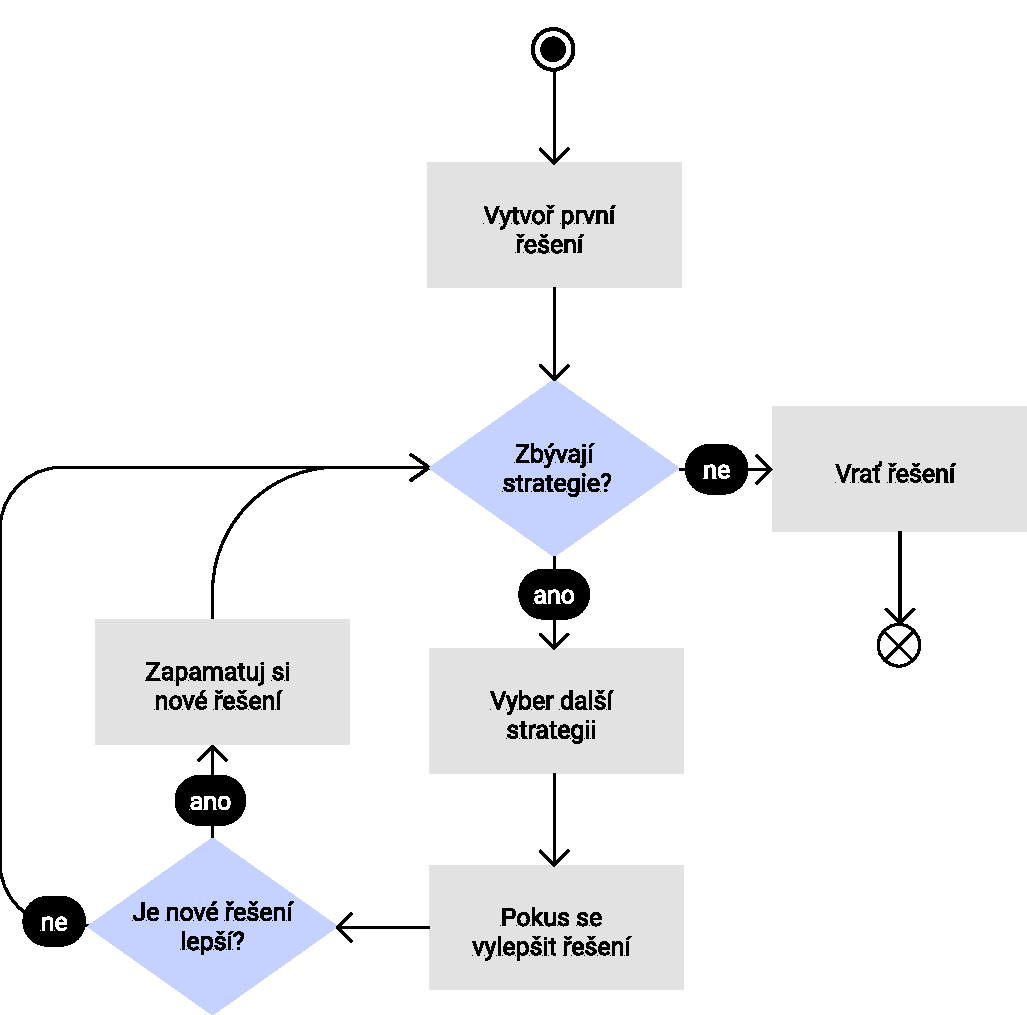
\includegraphics[scale=0.7]{img/algorithm-flow.pdf}
% 	\caption{Vývojový diagram algoritmu}
% 	\label{fig:algorithmflow}
% \end{figure}

\begin{lstlisting}[caption={Pseudokód rozvrhovacího algoritmu}, label={lst:scheduling}]
Vytvoř první řešení
POKUD zbývají strategie
	Zvol další strategii
	Pokus se vylepšit řešení
	POKUD je nové řešení lepší
		Ulož nové řešení
JINAK
	Vrať nejlepší řešení
\end{lstlisting}

Referenční řešení se se znalostí informací relevantních pro danou zbytnou podmínku algoritmus dále pokouší zlepšovat (postupně z hlediska různých podmínek).

Tento algoritmus se inspiruje u výše zmíněných řešení nalezených v~literatuře především v~podmínkách a v~zavedení náhodného referenčního řešení, které se postupně zlepšuje různými operacemi se sousedními strukturami, rovněž existencí vah a cílové funkce. Liší se především tím, že v~jednu chvíli je pro zjednodušení vylepšována a vyhodnocována právě jedna podmínka dle vlastní strategie, a to jen v~těch částech rozvrhu, kde dochází k~jejímu výraznému porušování (pokud tedy některé části rozvrhu danou podmínku nezhoršují, nejsou pro danou strategii relevantní). Po konci strategie se vyhodnocuje celkové řešení s~ohledem na váhy všech podmínek.

\subsection{Nepřekrývání směn, přestávka}
Ze zjevných důvodů nelze rozvrh vytvořit tak, aby byl jeden zaměstnanec přiřazen na více směn v~jednu chvíli. Z~legislativních požadavků navíc vyplývá nutnost mít mezi koncem jedné směny a začátkem další alespoň 11 hodin nepřetržitého odpočinku (u nezletilých zaměstnanců jde o 12 hodin), tímto tedy je rozšířena podmínka nepřekrývání směn. Pro jednoduchou ilustraci tohoto problému na třech dnech viz obr.~\ref{fig:shiftprecedencefull} (červená značí minimální přestávku).

\begin{figure}[h!]
	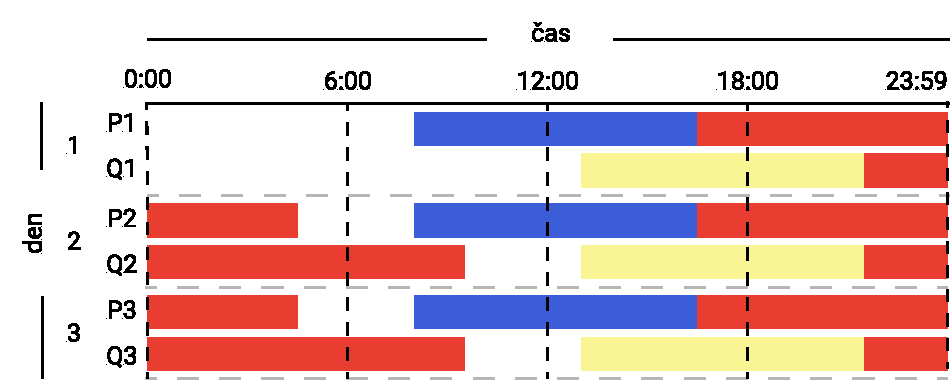
\includegraphics[scale=0.7]{img/shift-overlap.pdf}
	\caption{Nepřekrývání směn}
	\label{fig:shiftprecedencefull}
\end{figure}

Pro zjednodušení se v~tomto algoritmu pracuje s~grafem naznačeným na obr.~\ref{fig:shiftprecedence}, je možné v~něm vyhledávat platné kombinace směn o~nějaké délce, aby se směny nepřekrývaly.

\begin{figure}[h!]
	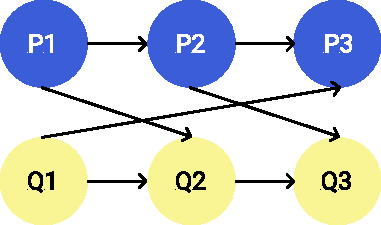
\includegraphics[scale=0.7]{img/shift-overlap-small.pdf}
	\caption{Graf následnosti směn}
	\label{fig:shiftprecedence}
\end{figure}


\section{Délka pracovního týdne}
Předpoklad pro algoritmus je co se týče délky pracovního týdne jednoduchý, neřeší možnost plánování přesčasů. Aby byla dodržena délka pracovního týdne (standardně 40 hodin), případně méně (zkrácené úvazky), každému zaměstnanci se rozvrhne nejvýše \texttt{úvazek $\ast$ 40 / délka směny} směn (zaokrouhleno nahoru). Když se směny ukládají, jedna náhodná z~nich se, je-li to třeba, zkrátí, aby byla délka pracovního týdne dodržena.

\section{Přiřazení na specializovanou směnu}

Pro každou specializovanou směnu existuje směna bez specializace, která probíhá ve stejný čas. Zaměstnanec může být přiřazen na libovolnou nespecializovanou směnu nebo na směnu se specializací odpovídající jeho smlouvě.

\section{Obsazení všech směn}
Tato strategie se pokouší do rozvrhu náhodně vybraných zaměstnanců vložit směnu, která zatím nebyla obsazena, a to způsobem popsaným v~pseudokódu~\ref{lst:noemptyshifts}. Tento algoritmus proběhne pro každou směnu nejvýše $n$-krát.

% \begin{figure}
% 	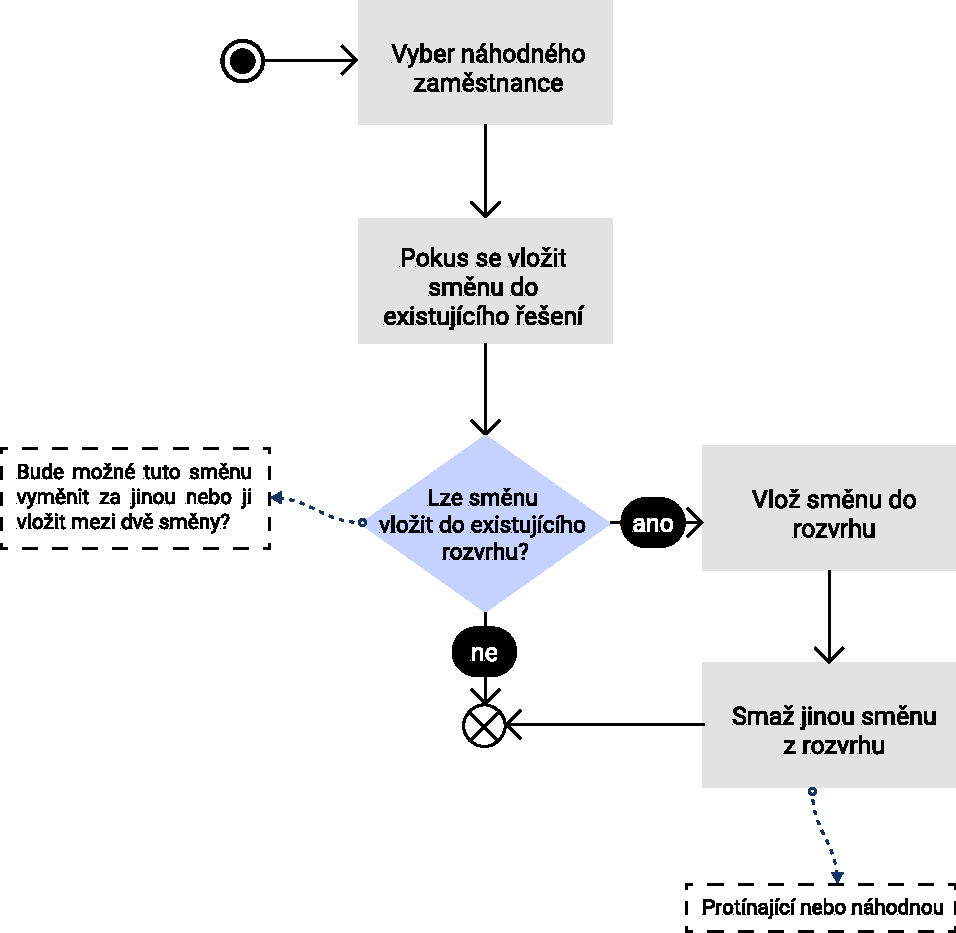
\includegraphics[scale=0.7]{img/no-empty-shifts.pdf}
% 	\caption{Strategie pro obsazení všech směn}
% 	\label{fig:noemptyshifts}
% \end{figure}


\begin{lstlisting}[caption={Strategie pro vylepšování obsazení všech směn}, label={lst:noemptyshifts}]
Vyber náhodného zaměstnance
POKUD lze vložit směnu do existujícího rozvrhu
	Vlož směnu do rozvrhu
	Smaž protínající nebo náhodnou směnu z rozvrhu
\end{lstlisting}


%Základní testování proběhlo na období jednoho týdne (o 7 pracovních dnech), v němž jsou rozepsány 3 směny mezi 8:00 a 22:30 (8hodinové s 30minutovou přestávkou), a to na 5, 10 a 20 zaměstnancích. Zatímco efekt u 20 zaměstnanců byl nepatrný (i v~náhodném řešení se směny mohly rozložit tak, že k porušování nedocházelo), v~případě menšího počtu zaměstnanců (10 a 5) vždy došlo ke snížení sankce, a tedy ke zlepšení oproti náhodnému řešení.

% \todo{Mám tohle rozpracovaný i pro další varianty -- testy mi běžely a výsledky mám}

% \begin{table}[h!]
% \begin{tabular}{|c|c|c|}
% 	\hline
% 	Zaměstnanců & Náhodné & Vylepšované \\
% 	& [průměr] & [průměr] \\
% 	\hline
% 	20 & 7,5 & 0 \\
% 	10 & 34,5 & 0 \\
% 	5 & 84 & 13 \\
% 	\hline
% \end{tabular}
% 	\caption{Testování na kombinaci specializovaných a nespecializovaných směn při sankci 10 za porušení}
% 	\label{tab:noemptyunspecialized}
% \end{table}
%
% Druhé testování této podmínky proběhlo na skupině 10 zaměstnanců s~úvazkem 1, kteří měli určenou specializaci. Rozvrhovalo se několik směn s relevantní specializací. Výsledky testování (pro souhrn viz tab.~\ref{tab:noemptyspecialized} ukázaly, že i~v~tomto případě dojde ke zlepšení, není ovšem tak výrazné, zvlášť v~případě, že všechny směny jsou specializované. Pravděpodobnou příčinou tohoto je nedostatečná implementace vyhledávání schémat specializovaných směn.
%
% \begin{table}[h!]
% 	\caption{Testování na specializovaných i nespecializovaných směnách při sankci 10 za porušení}
% 	\label{tab:noemptyspecialized}
% 	\begin{tabular}{|c|c|c|}
% 		\hline
% 		Specializovaných/ & Náhodné & Vylepšované \\
% 		Nespecializovaných & [průměr] & [průměr] \\
% 		\hline
% 		21/0 & 37,5 & 16 \\
% 		11/10 & 40 & 4 \\
% 		10/21 & 105 & 11 \\
% 		\hline
% 	\end{tabular}

%\end{table}

\section{Obsazení specializovaných směn}
Tato strategie změní přiřazenou směnu na specializovanou, která probíhá v~daném čase, je-li to možné vzhledem ke specializaci zaměstnance, viz pseudokód~\ref{lst:specialize} (průběh pro jednu směnu v~rozvrhu jednoho zaměstnance).

\begin{lstlisting}[caption={Strategie pro obsazení specializovaných směn}, label={lst:specialize}]
Vyber směnu bez specializace
POKUD probíhá ve stejný čas vhodně specializovaná směna
	Vyměň směnu za specializovanou
\end{lstlisting}


% \begin{figure}
% 	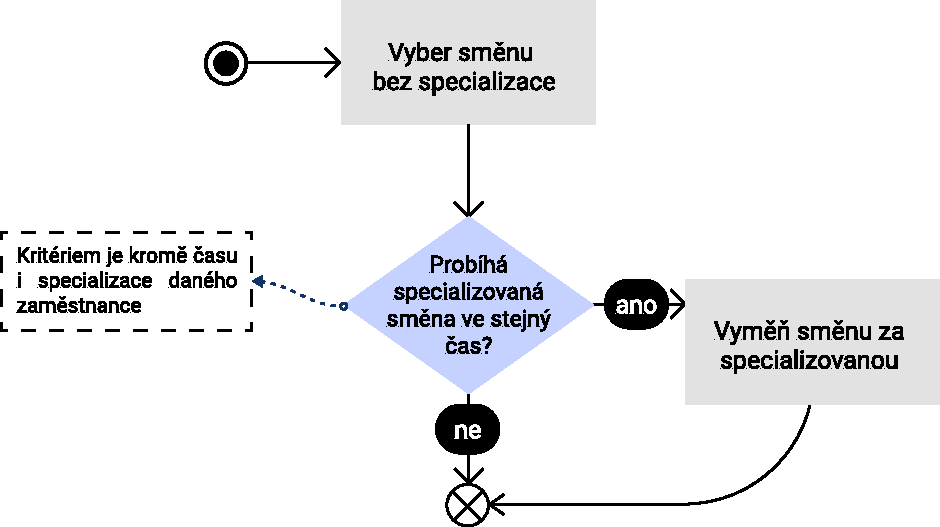
\includegraphics[scale=0.7]{img/specialize.pdf}
% 	\caption{Vývojový diagram pro obsazení specializovaných směn}
% 	\label{fig:specialize}
% \end{figure}

% \paragraph{Testovací data}
% \begin{table}[h]
% 	\caption{Testovací data}
% 	\label{tab:test-data-specialize}
% 	\begin{tabular}{l|l l l l l l }
% 		\hline
% 		  & dny & začátek & konec & délka & přestávka & směn\\
% 			\hline
% 			\rowcolor{Gray}
% 			A & 1–7 & 8:00 & 22:30 & 8 h & 30 min & 3  \\
% 		\hline
% 	\end{tabular}
% \end{table}
%
% \paragraph{Testovací data}
% \begin{table}[h]
% 	\caption{Testování}
% 	\label{tab:test-data-specialize-result}
% 	\begin{tabular}{l|l l l l l l }
% 		\hline
% 		  data & zam. & specializace & směny & sankce & náhodné & vylepšované\\
% 			\hline
% 			\rowcolor{Gray}
% 			 A & 16 & 8 S1, 8 S2 & 21 S1, 21 S2, 21 -  & 10 &  384 & 0 \\
% 		\hline
% 	\end{tabular}
% \end{table}

Úspěch této strategie je zaručen u všech směn, pro něž lze nalézt specializovanou směnu, která probíhá ve stejný čas – v~případě, že všechny směny lze specializovat, je sankce za porušení této podmínky vždy nulová. To ale znamená, že některé směny zůstanou zcela prázdné – tedy že naopak tato strategie může zhoršit obsazení všech směn  (je ale otázkou, jestli tento fakt má takovou váhu v~reálném světě a zda vůbec dává možnost \uv{na tuto směnu může přijít kdokoliv} smysl v~případě, že se směny mají rozepisovat s~ohledem na specializaci zaměstnanců).

\section{Více volna v~kuse}
Postup pro vylepšení, který se aplikuje na rozvrh každého zaměstnance, který zatím nemá 48hodinovou přestávku mezi směnami, je popsán v~pseudokódu~\ref{lst:freedays}. Především tento algoritmus jednu směnu odstraní (tím vytvoří delší volno), a poté se pokusí umístit další směnu mezi dvě jiné.

\begin{lstlisting}[caption={Strategie pro více volna v~kuse}, label={lst:freedays}]
Nalezni 48h přestávku mezi N-1 směnami
Odstraň směnu v tomto časovém období
POKUD lze směnu vložit do druhé největší přestávky
	Vlož směnu do této přestávky
\end{lstlisting}

% \begin{figure}
% 	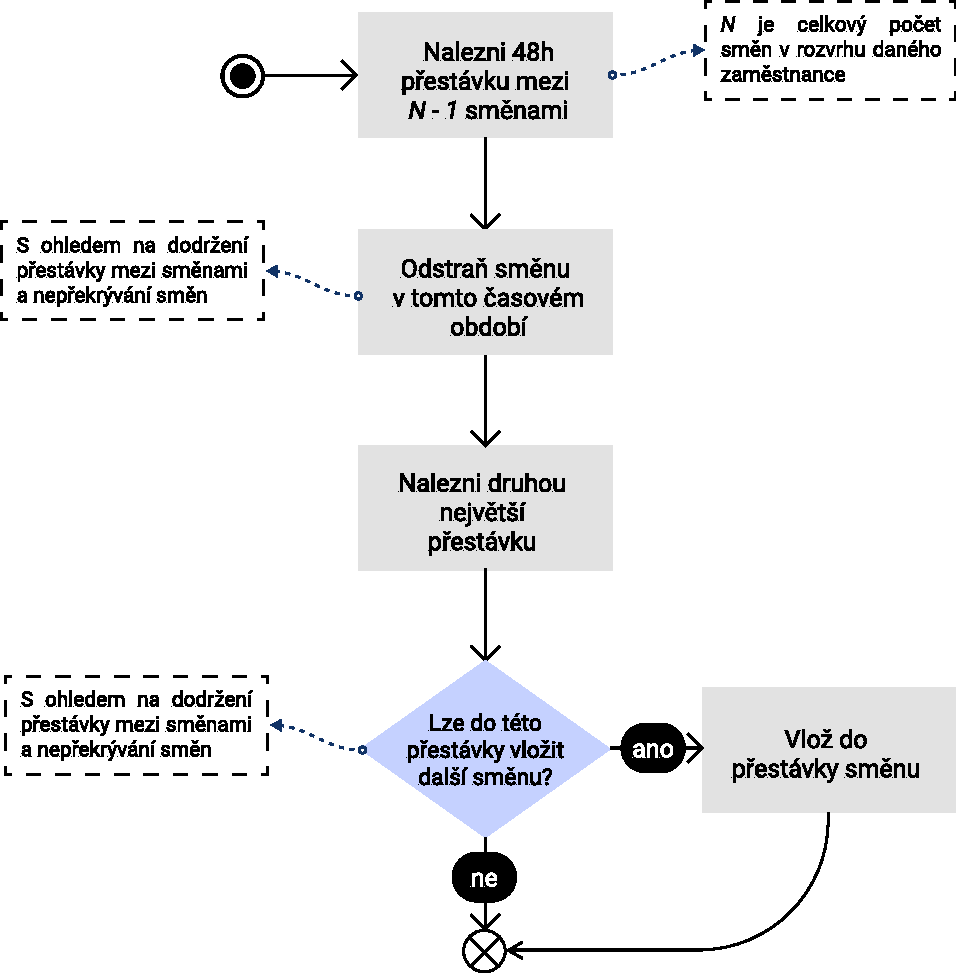
\includegraphics[scale=0.7]{img/free-days.pdf}
% 	\caption{Vývojový diagram pro obsazení specializovaných směn}
% 	\label{fig:freedays}
% \end{figure}

\section{Obsazení směn úměrně poptávce}
Nalezne se zaměstnanec, který je zapsán na směnu, kde naplnění převyšuje poptávku a $n$ náhodných směn, které poptávku nenaplňují – snahou je vyměnit přeplněnou směnu za prázdnější (pseudokód~\ref{lst:demand}).

\begin{lstlisting}[caption={Strategie pro obsazení směn dle poptávky}, label={lst:demand}]
Vyber náhodného zaměstnance na směnu
POKUD lze tuto směnu vyměnit za méně obsazenou
	Vyměň směnu za méně obsazenou
\end{lstlisting}

\section{Testování}

Při testování heuristických algoritmů nelze kontrolovat, zda byl vrácen jeden konkrétní výsledek (mimo jednoduché případy) a je možné pouze určovat, zda je řešení dost dobré, dost rychlé a validní. Může proběhnout sběr testovacích dat z~místa reálného nasazení algoritmu, případně mohou být data generována náhodně. \cite{rardin2001experimental}

Cílem bylo ověřit na několika sadách testovacích dat následující předpoklady:
\begin{enumerate}
	\item Algoritmus vrací pro validní vstupy validní řešení.
	\item Dochází ke zlepšení řešení, pokud proběhne alespoň jedna strategie.
	\item Pokud proběhnou všechny strategie, bude řešení nejlepší.
	\item Pokud má podmínka vyšší váhu, bude její zlepšení výraznější.
	\item Čím více iterací zlepšování, tím lepší řešení.
\end{enumerate}

Co se prvního předpokladu týče, řešení bude považováno za validní, pokud algoritmus proběhne bez vyvolání výjimky a bez zacyklení a pokud se řešení podaří uložit do databáze. Ve zbytku bude vyhodnocováno řešení jako celek po dokončení algoritmu~–~rozhodující bude počet porušení jednotlivých podmínek. Porovnáno bude náhodné a vylepšované řešení, konkrétně průměrný počet sankcí s~přihlédnutím ke standardní odchylce. Všechny testy proběhly desetkrát, souhrn je součástí přílohy \todo{Výsledky testování příloha}.

Z~výsledků testování lze jednoznačně říci, že řešení není horší než náhodné v~případě, že proběhne některá ze strategií.

Při testování algoritmu bylo zjištěno, že nevrací žádné řešení v~případě, že všechny směny bez specializace mají nulovou poptávku a někteří zaměstnanci mohou z~tohoto důvodu vzhledem ke své specializaci pracovat pouze méně směn v~daném týdnu. Je otázkou, zda toto považovat za správnou reakci na nevalidní vstupy, tedy pravděpodobně za chybu manažera, který si neuvědomil, že směny takto rozvhrnout nelze, případně zda je algoritmus vhodné opravit rozvrhnutím menšího množství směn (nesprávné řešení vzhledem k~pracovní době) nebo přiřazením směn s~nulovou prioritou či jinou specializací (nesprávné řešení vzhledem k~podmínkám algoritmu).

%Jednoduchým řešením by mohlo být zkrácení pracovního týdne podle specializace směn (vhodné řešení z~hlediska podmínek algoritmu), případně rozvržení i~nespecializovaných směn s~nulovou prioritou (vhodné řešení z~hlediska pracovní doby).


\section{Vyhodnocení algoritmu}

Byl navržen triviální algoritmus na rozdělení předem určených směn mezi zaměstnance s~různě velkým úvazkem. V~případě budoucího použití by bylo třeba dále jej vylepšit a vzít v~potaz, co by od rozvrhovacího algoritmu očekával ten, kdo by jej využival~–~skoro jistě by se jednalo o~složitější optimalizační úlohu, která by vyžadovala odlišný model.


\chapter{Implementace}

\section{Architektura aplikace}

Při implementaci byla použita třívrstvá architektura (klient, aplikační server, databáze), jak je naznačeno na obr.~\ref{fig:architecture}. Klientem zde je mobilní aplikace, která komunikuje se serverem přes jeho REST API. Serverová aplikace běží v Dockeru z~důvodu snazšího nasazení na různá prostředí.

Kromě samotné Rails aplikace a databáze jsou v~Dockeru i kontejnery Redis a~Sidekiq, a to z~důvodu zpracování operací na pozadí, v~této aplikaci jde především o~pravidelné~vytvoření nového týdne pro rozvrhnutí nebo zveřejnění rozvrhu v~případě, že to vedoucí neudělá v~dostatečném předstihu.

Mimo tuto strukturu stojí Firebase Cloud Messaging, který se používá pro posílání notifikací (např.~o~zveřejnění nového rozvrhu nebo nového týdne na naplánování) do mobilní aplikace, když si toto server vyžádá.

\begin{figure}[h]
	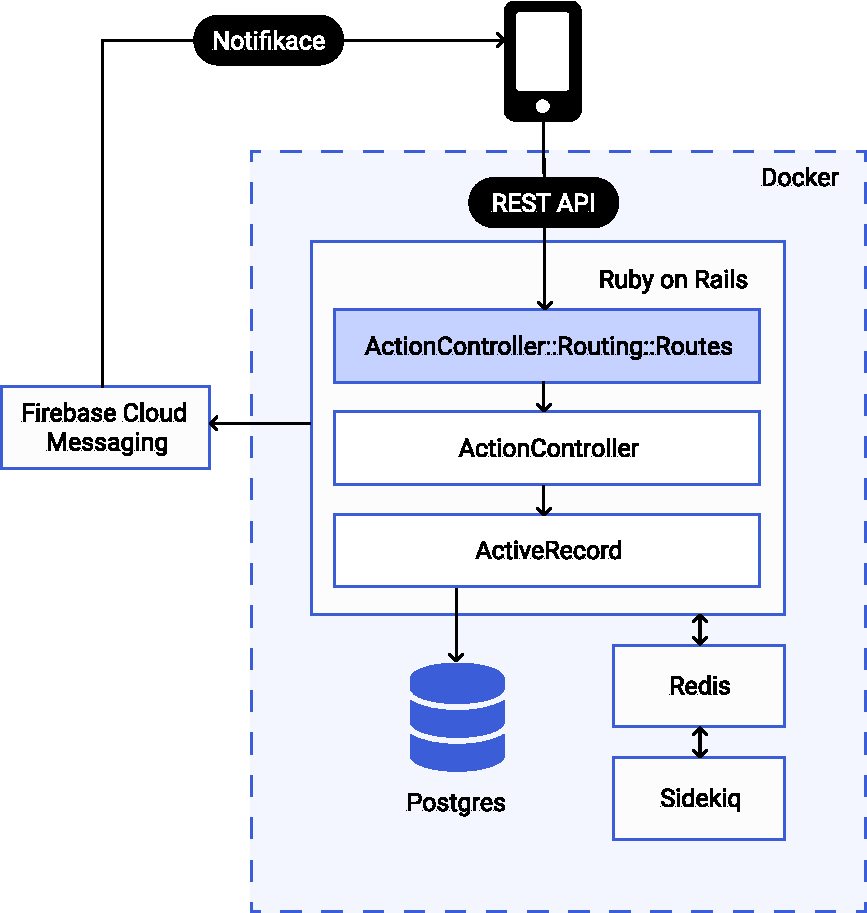
\includegraphics[scale=0.7]{img/architecture.pdf}
	\caption{Architektura aplikace}
	\label{fig:architecture}
\end{figure}

\section{Backend}

Backendová aplikace využívá architektonický vzor MVC, přičemž uživatelské rozhraní (view) je zcela zajištěno mobilní aplikací, a není tedy součástí webové aplikace.

Aplikace byla implementována tak, aby byly dodrženy konvence a nebylo třeba ji příliš konfigurovat~–~controllery jsou implementovány na základě konvencí, není-li nutné to udělat jinak, tzn.~že v~případě, že přijde požadavek \texttt{GET /resources}, provolá se metoda \texttt{index} v~\texttt{ResourceController} (jedna z~konvencí v~Rails), model je implementován s~pomocí objektově relačního mapování, které se stará o~přístup k~databázi. Mimo strukturu specifickou pro webovou aplikaci stojí \texttt{Service} třídy, které se provolávají v~případě, že je vhodné některé akce odsunout mimo Controller, a také pomocné datové struktury a strategie pro rozvrhování směn.

Používají se především gemy\footnote{Gem je termín pro knihovny v~Ruby.} Devise Token Auth (autentizace uživatele s~pomocí tokenů), CanCanCan (zabezpečení operací se zdroji na základě uživatelské role) nebo will paginate (stránkování zdrojů).

Diagram tříd je součástí přílohy \ref{sec:diagram}.

\section{Mobilní aplikace}

Mobilní aplikace byla navrhnuta dle zásad nejpoužívanější a ze stranu Googlu doporučovaného architektonického vzoru MVVM. Při implementaci byly využity především knihovny Koin (pro dependency injection), Retrofit (HTTP klient) a dále některé součásti Android Jetpack (soubor knihoven pro platformu Android, které usnadňují vývoj udržitelných aplikací a poskytují kompatibilitu se staršími verzemi OS \cite{android2020jetpack}), a to především LiveData (pozorovatelná data respektující životní cyklus Android UI komponent), Navigation (navigace mezi fragmenty aplikace), DataBinding (propojení UI komponent definovaných v~XML~layoutech s~daty), Paging (stránkování seznamů) nebo Room (nadstavba nad databázi SQLite pro perzistenci dat).

Jedná se o~aplikaci s~nižším počtem aktivit (samostatné aktivity se využívají v~případě, že by nebylo vhodné zobrazovat v~aplikaci spodní navigaci, což znamená tehdy, když se vytváří nové zdroje, např.~nový zaměstnanec), v~níž navigace probíhá s~pomocí komponenty Navigation (např. detaily směn tedy nejsou sa\-mos\-tat\-ný\-mi aktivitami, ale jedná se o~fragmenty v~aktivitě \texttt{MainActivity}). Tento přístup k~navigaci byl odpozorován např.~u aplikací Spotify, YouTube nebo Instagram.


% \subsection{View}
%
% View je ta část aplikace, která vykresluje uživatelské rozhraní, může se jednat o~layouty ve formátu XML, aktivity nebo fragmenty. Má referenci na ViewModel a pozoruje jeho změny, podle čehož aktualizuje UI; při událostech na uživatelském rozhraní (např.~stisknutí tlačítka) může provolat ViewModel.
%
% \subsubsection{Layout}
%
% Layout definuje strukturu uživatelského rozhraní, kde jsou na obrazovce jaké prvky a jak tyto prvky vypadají; lze ho deklarovat v~souboru formátu XML (pak je třeba tento layout propojit s~aktivitou/fragmentem) nebo za běhu programu, případně s~pomocí knihovny Jetpack Compose. \cite{android2020layouts}
%
% \subsubsection{Aktivita}
%
% Aktivita (rozšíření třídy \texttt{android.app.Activity}) je základní stavební blok Android aplikace, jedná se o \uv{okno}, do nějž se vykresluje uživatelské rozhraní. Aktivity mají svůj životní cyklus, který se řídí především podle toho, zda zrovna jsou viditelné pro uživatele. Ničení aktivit (destroy) řídí operační systém. \cite{android2020activity}
%
% \subsubsection{Fragment}
%
% Fragment je znovupoužitelná část uživatelského rozhraní, která má svůj vlastní životní cyklus i layout; narozdíl od aktivity ale nemůže existovat samostatně -- musí být vložen do aktivity. \cite{android2020fragments}
%
% \subsection{ViewModel}
%
% ViewModel interaguje s~modelem, na základě dat, která mu model vrátí, mění stav svých proměnných.
%
% \subsection{Model}
%
% Model se často skládá z~repozitářů (jedná se o~běžný způsob návrhu, nikoli o přímou součást platformy), které dále provolávají datové zdroje (lokální či vzdálené) a poskytuje tak požadovaná data.


\subsection{View}

View je část aplikace, která vykresluje uživatelské rozhraní, může se jednat o~layouty ve formátu XML, aktivity (základní okno pro UI) nebo fragmenty (znovupoužitelné). Má referenci na ViewModel a pozoruje jeho změny, podle čehož aktualizuje UI; při událostech na uživatelském rozhraní (např.~stisknutí tlačítka) může provolat ViewModel.

Pro zjednodušení se používá data binding --  vytváření nových aktivit byla vytvořena abstraktní třída \texttt{BindingActivity<B: ViewDataBinding>}. Abstraktní aktivita nastaví layout a binding, který je pro potomky přístupný jako proměnná \texttt{binding}, a~nastaví mu vlastníka životního cyklu.

Třída \texttt{ViewModelActivity<V: BaseViewModel, B:  ViewDataBinding>} je abstraktnim potomkem \texttt{BindingActivity}, který je přípraven pro aktivity, které mají vazbu na ViewModel (parametry konstruktoru jsou layout a třída ViewModelu). Tato aktivita zajišťuje vytvoření ViewModelu (který se uloží do proměnné \texttt{viewModel} a navíc se nastaví jako parametr pro binding).

Velmi podobně jako \texttt{BindingActivity} a \texttt{ViewModelActivity} fungují také abstraktní fragmenty, tj. \texttt{BindingFragment} a \texttt{ViewModelFragment}.

Vzhledem k~použití knihovny LiveData (pozorovatelná data závislá na životním cyklu aktivity/fragmentu) zde větší míře použit návrhový vzor Observer, View pozoruje změny ViewModelu a podle toho se mění obrazovky.

\subsection{ViewModel}

ViewModel je prostředníkem mezi aktivitou a~modelem -- provolává nižší vrstvu a na základě dat, která mu vrátí, mění stav svých proměnných.

ViewModely jsou v~této aplikaci potomkem abstraktní třídy \texttt{BaseViewModel}, která v~sobě obsahuje odkazy na všechny repositáře (inicializace je tzv. \textit{lazy}, s~pomocí dependency injection); také obsahuje LiveData pro zobrazování chyb a metody pro zpracování chyb a dat (to vše proto, aby se méně opakoval stejný kód). ViewModel ukládá odpovědi z~repozitářů jako LiveData (obecně by repozitáře měly být odstíněny od specifik platformy).

\subsection{Model}
Model se často skládá z~repozitářů (jedná se o~běžný způsob návrhu, nikoli o přímou součást platformy), které dále provolávají datové zdroje (lokální či vzdálené) a poskytuje tak požadovaná data. Tímto způsobem je implementována i v~této aplikaci -- repozitáře mají zodpovědnost za provolání správných datových zdrojů a za ukládání dat do databáze či do cache. Odpovědi se vracejí obalené ve třídě \texttt{ResponseModel<T>} (viz kód~\ref{lst:responsemodel}), která může nést zprávu o chybě nebo požadovaná data.

\begin{lstlisting}[language=Kotlin,caption={Třída \texttt{ResponseModel}},label={lst:responsemodel}]
sealed class ResponseModel<T> {
	class SUCCESS<T>(var data: T? = null, val headers: Headers? = null): ResponseModel<T>()

	class ERROR<T>(val errorType: ErrorType? = null): ResponseModel<T>()
}
\end{lstlisting}

\section{Design}\label{design}

Design aplikace vznikl v souladu se základními pravidly Material Designu. Snahou bylo vytvořit minimalistické, jednoduché uživatelské rozhraní~--~vzhled uživatelského rozhraní byl navrhnut v~nástroji Figma. Ikonky byly převzaty z~knihoven Font Awesome 5 (fas) a Material Design Icon (mdi). Pro konkrétní návrhy viz~přílohu \ref{sec:ui}.

\chapter*{Závěr}


\printbibliography[title={Seznam použité literatury}]

\appendix

\chapter{Internetové odkazy}
\section{Uživatelské příběhy}\label{sec:user-story}

Mapa uživatelských příběhů v plné velikosti
\begin{itemize}
	\item \url{https://github.com/kopemar/baka-docs/blob/main/storyboard.pdf}
\end{itemize}


\section{Návrh uživatelského rozhraní}\label{sec:ui}

Wireframes, mapa obrazovek v mobilní aplikaci
\begin{itemize}
	\item \url{https://github.com/kopemar/baka-docs/blob/main/lfp.pdf}
\end{itemize}


Design obrazovek \todo{Příloha design}
\begin{itemize}
	\item \url{https://github.com/kopemar/baka-docs/blob/main/lfp.pdf}
\end{itemize}


\section{Zdrojové kódy}

Mobilní aplikace
\begin{itemize}
	\item \url{https://github.com/kopemar/baka-android}
\end{itemize}

Backend aplikace
\begin{itemize}
	\item \url{https://github.com/kopemar/baka-api}
\end{itemize}

\newpage

\section{Diagramy}\label{sec:diagram}

Diagram tříd
\begin{itemize}
	\item \url{https://github.com/kopemar/baka-docs/blob/main/class_diagram.pdf}
\end{itemize}

\end{document}
